\chapter{Structured Mining}\label{ch:StructuredMining}
  Motivated by the declarative modeling paradigm for data mining, we report on our experience in modeling and solving relational query and graph mining problems with the IDP system, a variation on the answer set programming paradigm. Using IDP or other ASP-languages for modeling appears to be natural given that they provide rich logical languages for modeling and solving many search problems and that relational query mining (and ILP) is also based on logic.

  Nevertheless, our results indicate that second order extensions to these languages are necessary for expressing the model as well as for efficient solving, especially for what concerns subsumption testing. We propose such second order extensions and evaluate their potential effectiveness with a number of experiments in subsumption as well as in query mining.




\section{Introduction}
\label{sec:intro}
In the past few years, many pattern mining problems have been modeled using constraint programming techniques \parencite{guns_framework}.
While the resulting systems are not always as efficient as state-of-the-art pattern mining systems,
the advantages of this type of declarative modeling are  now generally accepted: they support more constraints,
they are easier to modify and extend, and they are built using general purpose systems.
However, so far, the declarative modeling approach has not yet been applied to inductive logic programming. This chapter investigates whether such 
an extension would be possible.  To realize this, we consider frequent query mining, the ILP version of frequent pattern mining, as well as the answer set programming paradigm, the logic programming version of constraint programming. 
More specifically, we address the following three questions: 

\begin{enumerate}
\item[\qone] Is it possible to design and implement a declarative query miner that uses a logical and relational representation for both the data and the query mining problem? 
\item[\qtwo] Is it possible to take advantage of recent progress in the field of computational logic by adopting an Answer Set Programming (ASP) \parencite{eiter} framework for modeling and solving? 
\item[\qthree] Would such a system be computationally feasible? That is, can it tackle problems of at least moderate size?
\end{enumerate}
Our study is not only relevant to ILP, but also to the field of knowledge representation and ASP
as query mining (and ILP) is a potentially interesting application 
that may introduce new challenges and suggest solver extensions. 

More concretely, the main contributions of this work can be summarized as follows:
\begin{enumerate}
  \item We present two declarative models and corresponding solving strategies for the query mining problem that support a wide variety of constraints.  While one model can be expressed in the ASP paradigm, the other model requires a  second order extension that we believe
to be essential for modeling ILP tasks. 
  \item We implement and evaluate the presented models in the IDP system \parencite{idp}, a knowledge base system that belongs to the ASP paradigm.
  \item We empirically evaluate the proposed models and compare them on the classical datasets with the state-of-the-art ILP methods.
\end{enumerate}


\section{Problem statement}\label{sec:problem}

The problem that we address in this chapter is to mine queries in a logical and relational learning setting. Starting with the work the Warmr system \parencite{warmr}, there has been a line of work that focusses on the following frequent query mining problem \parencite{bagm,farmer,condensed_luc}:


\noindent
{\bf Given:} \vspace{-8pt}
\begin{itemize}
\item a relational database $D$,
\item the entity of interest determining the \keypred/1 predicate,
\item a frequency threshold $t$,
\item a language ${\cal L}$ of logical queries of the form $\keypred(X) \leftarrow b_1, ..., b_n$ defining $key/1$ ($b_i$'s are atoms).
\end{itemize}\vspace{-5pt}
{\bf Find:} all queries $c \in {\cal L}$ s.t. $\freqpred(c,D) \geq t$, where 
\begin{equation*}
\freqpred(c,D) = |\{\theta \mid D \cup c \models key(X)\theta \}|.
\end{equation*}

Notice that the substitutions $\theta$ only substitute variables $X$ that occur in \keypred. 

In this chapter, we focus our attention on graph data, as this forms the simplest truly relational learning setting and allows us to focus on what is essential for extending the declarative modeling paradigm to a relational setting. In principle, this setting can easily be generalized to the full inductive logic programming problem. 
 
As an example, consider a graph database $D$, represented by the facts 
\begin{equation*}
\{ \edge(g_1,1,2),~ \edge(g_1,2,3),~ \edge(g_1,1,3),~ \edge(g_2,1,2),~ \edge(g_2,2,3),~ \edge(g_2,1,3), \dots \},
\end{equation*}
where the ternary relation $\edge(g,e_1,e_2)$ states that in graph $g$ there is an edge between $e_1$ and $e_2$ (we assume graphs to be undirected, so there is also always an edge between $e_2$ and $e_1$). The frequency of $\textit{key}(K) \leftarrow \edge(K,B,C), \edge(K,C,D), \edge(K,B,D)$ in this database is 2 as the query returns $g_1$ and $g_2$. If $key(g)$ holds,  then the graph $g$ is subsumed by the query specified defined in the body of the clause for \keypred.

The goal of this chapter is to explore how such typical ILP problems can be encoded in 
ASP languages.   So, we will need to translate the typical ILP or Prolog construction into an ASP format. 
In the present chapter, we employ ASP as well as IDP, which belongs to the ASP family of formalisms. Most statements and constraints written in IDP can be translated into standard ASP mechanically. %Any particular deviation from mainstream the ASP approach is indicated. 
A brief example-based introduction to IDP is in Appendix \ref{sec:idp_intro} and for a detailed system and paradigm description we refer to the IDP system and language description \parencite{idp} and to the ASP primer \parencite{eiter}.

To realize frequent query mining in IDP, we need to tackle four problems: 1) encode the queries in IDP; 2) implement the subsumption test to check whether a query subsumes a particular entity in the database; 3) choose and encode a language bias; and 4) determine, in addition to frequency, further constraints that could be used and encode them. We will now address each of these problems in turn.

\section{Encoding}\label{sec:encoding}
We assume that the dataset $D$ is encoded as two predicates $\edge(g,e_1,e_2)$, described before, and the ternary relation $\nodelabel(g,n,l)$ that states that there is a node $n$ with label $l$ in graph $g$ (for a discussion on how to extend the approach, see Section \ref{sec:approach_extension}) . 

\paragraph{Encoding a query}
The coverage test in ILP is often $\theta$- or  $OI$-subsumption.
%Typically in Prolog a subsumption test is encoded as an evaluation of a rule, which corresponds to the existence of a $\theta$ mapping. If such a mapping exists, then the homomorphism check is positive, otherwise it is negative. 

\begin{definition}[$OI$ and $\theta$-subsumption \parencite{luc_book}]
  A clause $c_1$ $\theta$-subsumes a clause $c_2$ iff there exists a substitution $\theta$ such that $c_1 \theta \subseteq c_2$. 
Furthermore, $c_1$ 
  OI-subsumes $c_2$ iff there exists substitution $\theta$ such that $\compl(c_1) \theta \subseteq \compl(c_2)$, where $\compl(c) = c \cup \{ t_i \neq t_j \mid t_i \textit{ and } t_j \textit{ are two distinct terms in c }\}$.
\end{definition}
 
As ASP and, in particular, IDP are model-generation approaches, they always generate a set of ground facts. This implies that ultimately the queries will have to be encoded by a set of ground facts for $\edge$ and $\nodelabel$ as well (e.g., $\{ \edge(q,77,78),~ \edge(q,77,79),$ $\nodelabel(q,77,a),~ \nodelabel(q,78,b),~ \nodelabel(q,79,c),\dots \}$)
%Under the assumption that we are working with graphs, a query $q$ is nothing else than a dedicated graph that would be encoded in a similar way. 
%\vspace{-6pt}
and that we need to explicitly encode subsumption testing, rather than, as in Prolog, simply evaluate the query on the knowledge base.  We use the convention that if a quantifier for a variable is omitted, then it is universally quantified. Furthermore, we use the convention that variables start with an upper-case and constants with an lower-case character. To illustrate the idea, consider the program in Eq. \ref{eq:full_subsumption} that has a model if and only if the query $q$ $OI$-subsumes the graph $g$.
If we remove the last constraint in Eq. \ref{eq:full_subsumption}, we obtain $\theta$-subsumption.
Notice that the function $\theta$ will be explicit in the model. 
This program can be executed in IDP directly.  

\begin{equation}
\begin{aligned}
  \edge(q,X,Y) &\implies \edge(g,\theta(X), \theta(Y)).  \\
  \nodelabel(q,X,L) &\implies \nodelabel(g,\theta(X),L) . \\
  X \neq Y &\implies \theta(X) \neq \theta(Y).
\end{aligned}
  \label{eq:full_subsumption}
\end{equation}

Notice that, in theory, it would be possible to simply encode subsumption testing 
in IDP or ASP as rule evaluation, that is, in the above example, to assert the knowledge base and to define the rule $\keypred$ and then to ask whether $\keypred(g)$ succeeds. 
Computationally, this would however be infeasible as the size of the grounded rules 
grows exponentially with the number of distinct variables in the rule.

Throughout the chapter we use OI-subsumption for all tasks, except of the experimental comparison with Subsumer in Section \ref{sec:experiments} (since, it is not designed to perform OI-subsumption).

\paragraph{Encoding the language bias}
In practice, one often bounds query languages, for instance by using a bottom clause and only considering queries or clauses that subsume the bottom clause. 

\begin{definition}[Language bias of a bottom clause $\bot$]
  Let $\bot$ be a clause that we call bottom, then the language bias $L$ is a set of clauses: $L = \{ c \mid c \textit{ OI-subsumes } \bot\}$.
\end{definition}

This approach also works for ASP. We select one graph from the data and the set of all atoms in that instance will serve as bottom clause $\bot$. When fixing such an instance, we can encode queries by listing the nodes in that entity that will be present in the pattern using the unary predicate $\invar(x)$ (for \textit{in query}), as visualized in Figure \ref{fig:single}.

We now present a modification of the previous encoding in Eq. \ref{eq:full_subsumption} that takes into account the selection of the subgraph of the picked graph $q$ as a query (marked in red in Figure \ref{fig:single}). We refer to the edges in the bottom clause as \tedge and labels in the bottom clause as \tlabel. When we refer to a node in the bottom clause, we call it a \textit{bnode}.
\begin{equation}
\begin{aligned}
  \invar(X) \wedge \invar(Y) \wedge \tedge(X,Y) &\implies \edge(g,\theta(X), \theta(Y)).  \\
  \invar(X) \wedge \tlabel(X,L) &\implies \nodelabel(g,\theta(X),L). \\
  \invar(X) \wedge \invar(Y) \wedge X \neq Y &\implies \theta(X) \neq \theta(Y).
\end{aligned}
  \label{eq:invar_single_subsumption}
\end{equation}
The intuition behind these rules is that we select a subgraph by picking nodes in the bottom clause (i.e., a graph), and then we enforce the constraints on the nodes that have been selected. Eq. \ref{eq:invar_single_subsumption} implements this by adding an \invar predicate at the beginning of each clause as a guard, the rule is activated iff the corresponding node is selected.
\
\paragraph{Encoding the multiple subsumption test}
In frequent query mining one is interested in mining \textit{frequent} queries, which implies that there is a bag of graphs to match. 

\begin{figure}[t]
  \begin{center}
    
  \begin{subfigure}{.44\textwidth}
    \captionsetup{
    }
    \begin{center}
      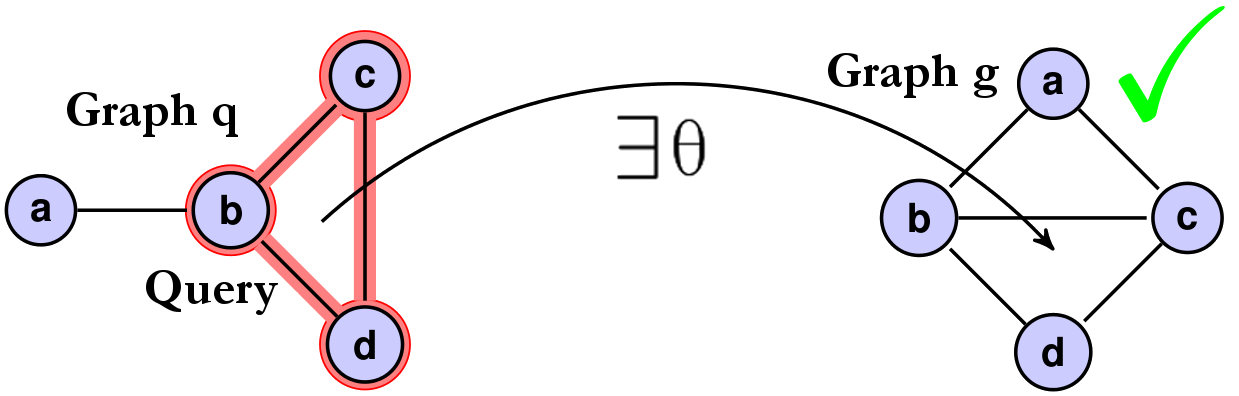
\includegraphics[width=1.0\textwidth]{figure_single.png}
      \caption{Single graph subsumption by a subgraph query ($\invar(x)$ in red)}
      \label{fig:single}
    \end{center}
    \hfill 
  \end{subfigure}
    \begin{subfigure}{.44\textwidth}
    \captionsetup{
    }
    \begin{center}

      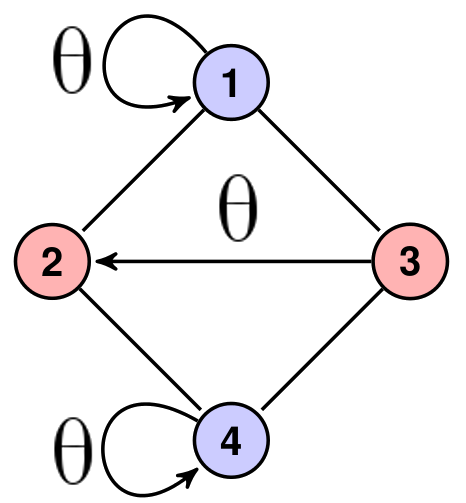
\includegraphics[width=0.33\textwidth]{figure_automorphism.png}
      \caption{Canonicity check: the subgraph on nodes 1-3-4 is mapped to 1-2-4 (lexicographically smaller)}
      \label{fig:automorphism}
    \end{center}
  \end{subfigure}
 
    \captionsetup{
    }
  \caption{Examples of single graph subsumption (left) and of a canonicity check (right)}
  \end{center}
\end{figure}
  
\paragraph{Frequent query enumeration in Algorithm \ref{algo:top_cycle}}
\begin{algorithm}[thb]
  \begin{algorithmic}
    \footnotesize
    \State \textbf{Input:} $D,k,t$ \Comment{Dataset, \#Queries, Threshold}
    \State \textbf{Output:} \patternset~-- set of frequent queries
    \State $\patternset \gets \emptyset$
    \State $\bot \gets \textit{pick-language-bias(D)}$ \Comment{Language bias obtained from data}
    \State $\maxsize \gets \#\textit{nodes}(\bot)$
    \State $i \gets 0$
    \For{$\size \in 1\dots\maxsize$}
    \State $\nogoods \gets \emptyset$
    \While{True} \label{algo:line:while}
    \State $\pattern \gets \getquery(D,\bot,t,\size,\nogoods)$ \Comment{IDP call, Eq. \ref{constr:fol_matching}}
    \If{\pattern is None}
    \State break \Comment{the line below: IDP call, adopted Eq. \ref{eq:canonical}}
  \EndIf 
  \State $\canon, \isoset \gets \getcanonicalform(\pattern, \bot)$ 
  \State $\patternset \gets \patternset \cup \{\canon\}$
  \State $\nogoods \gets \nogoods \cup \isoset$
  \State $i \gets i + 1$ 
  \If{$i \geq k$}
  \Return \patternset
\EndIf
  \EndWhile
\EndFor\\
\Return \patternset
\end{algorithmic}
\caption{First Order Model: Iterative Query Enumeration}
\label{algo:top_cycle}
\end{algorithm}
We enumerate all frequent queries starting from the smallest ones (with only 1 node) to the largest ones (the bottom clause). Algorithm \ref{algo:top_cycle} has two loops. The first sets the current query size and sets \mic to be empty (since we do not want to prohibit generation of supersets of already found queries). In the inner loop, we obtain a candidate for a frequent query by calling IDP once, then we check if the query is in canonical form and also obtain all isomorphic queries to this canonical form. After that we generate a \mic for each of them and prohibit the whole isomorphic class of queries to be generated. Note that generating all isomorphic queries is prohibitive, that is why we obtain a canonical query and remove all other isomorphic queries. The algorithm terminates if either it cannot find a new frequent query of any size or the required number of queries has been enumerated. 
\paragraph{Top-$k$ problem}
Current ASP solvers, including IDP, can perform optimization described in Constraints \ref{eq:max_size}, \ref{eq:coverage} and \ref{eq:discriminative_coverage}. However, Algorithm \ref{algo:top_cycle} enumerates patterns with respect to their size and therefore needs to be modified. The key change is to remove the outer \textit{for} loop with the size variable together with  \CardinalityConstraint. In the experiment section we demonstrate that even top-$1$ is already excessively complex for modern ASP solvers and requires further investigation and development of the systems. 

\section{Experiments}\label{sec:experiments}
\begin{figure}[t]
  \captionsetup{
    skip=-5pt
  }
  \begin{center}
    \begin{subfigure}{.39\textwidth}
      \captionsetup{
        font={scriptsize},
        skip= 0pt
      }
      \begin{center}
        \scalebox{0.8}{
          \begin{tabular}{l c c c c}
            \textbf{Name} & \textbf{Graphs} & \textbf{Vertices} & \textbf{Edges} & \textbf{Labels}\\
            Mutagenesis  & 230& 26& 27&  9\\
            Enzymes  & 600 & 33 & 124 &  3\\
            Toxinology  & 417& 26 & 26&  22\\
            Bloodbarr & 413 & 21  & 23& 9\\
            NCTRER & 232& 19& 20      & 9\\
            Yoshida & 265 & 20 & 23   &  9
          \end{tabular}
        }
      \end{center}
      \caption{Dataset description\\ (avg for vertices, edges, labels)}
      \label{table:datasets}
    \end{subfigure}
    \hfill
    \begin{subfigure}{.60\textwidth}
      \captionsetup{
        font={scriptsize},
        skip= 0pt
      }
      \phantom{-}
      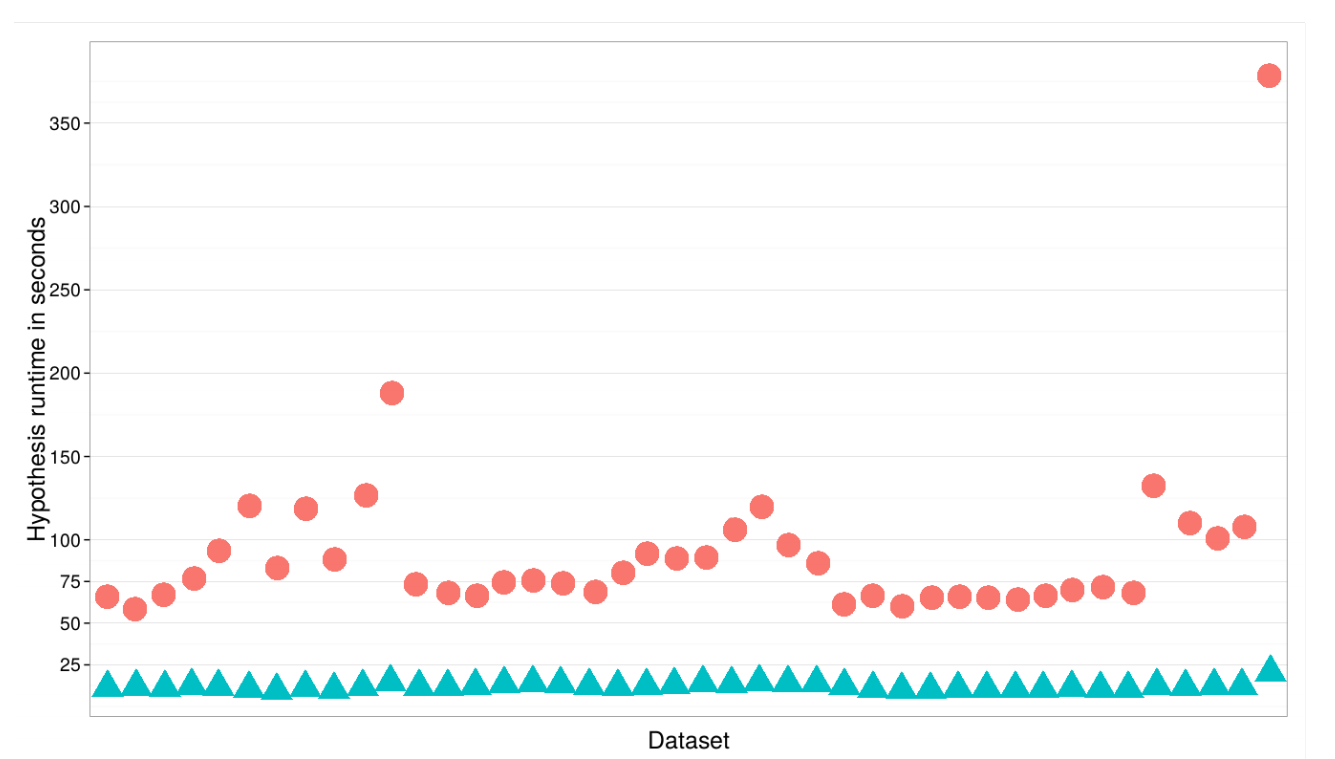
\includegraphics[width=1.03\linewidth]{subsumption.png}
      \caption{Single subsumption test. IDP (circles) and Subsumer (triangles) \\ (avg time per hypothesis in seconds; ILP phase transition datasets)}
      \label{figure:subsumption}
    \end{subfigure}
    \hfill 
    \begin{subfigure}{.70\textwidth}
      \captionsetup{
        font={scriptsize},
        skip=2pt
      }
      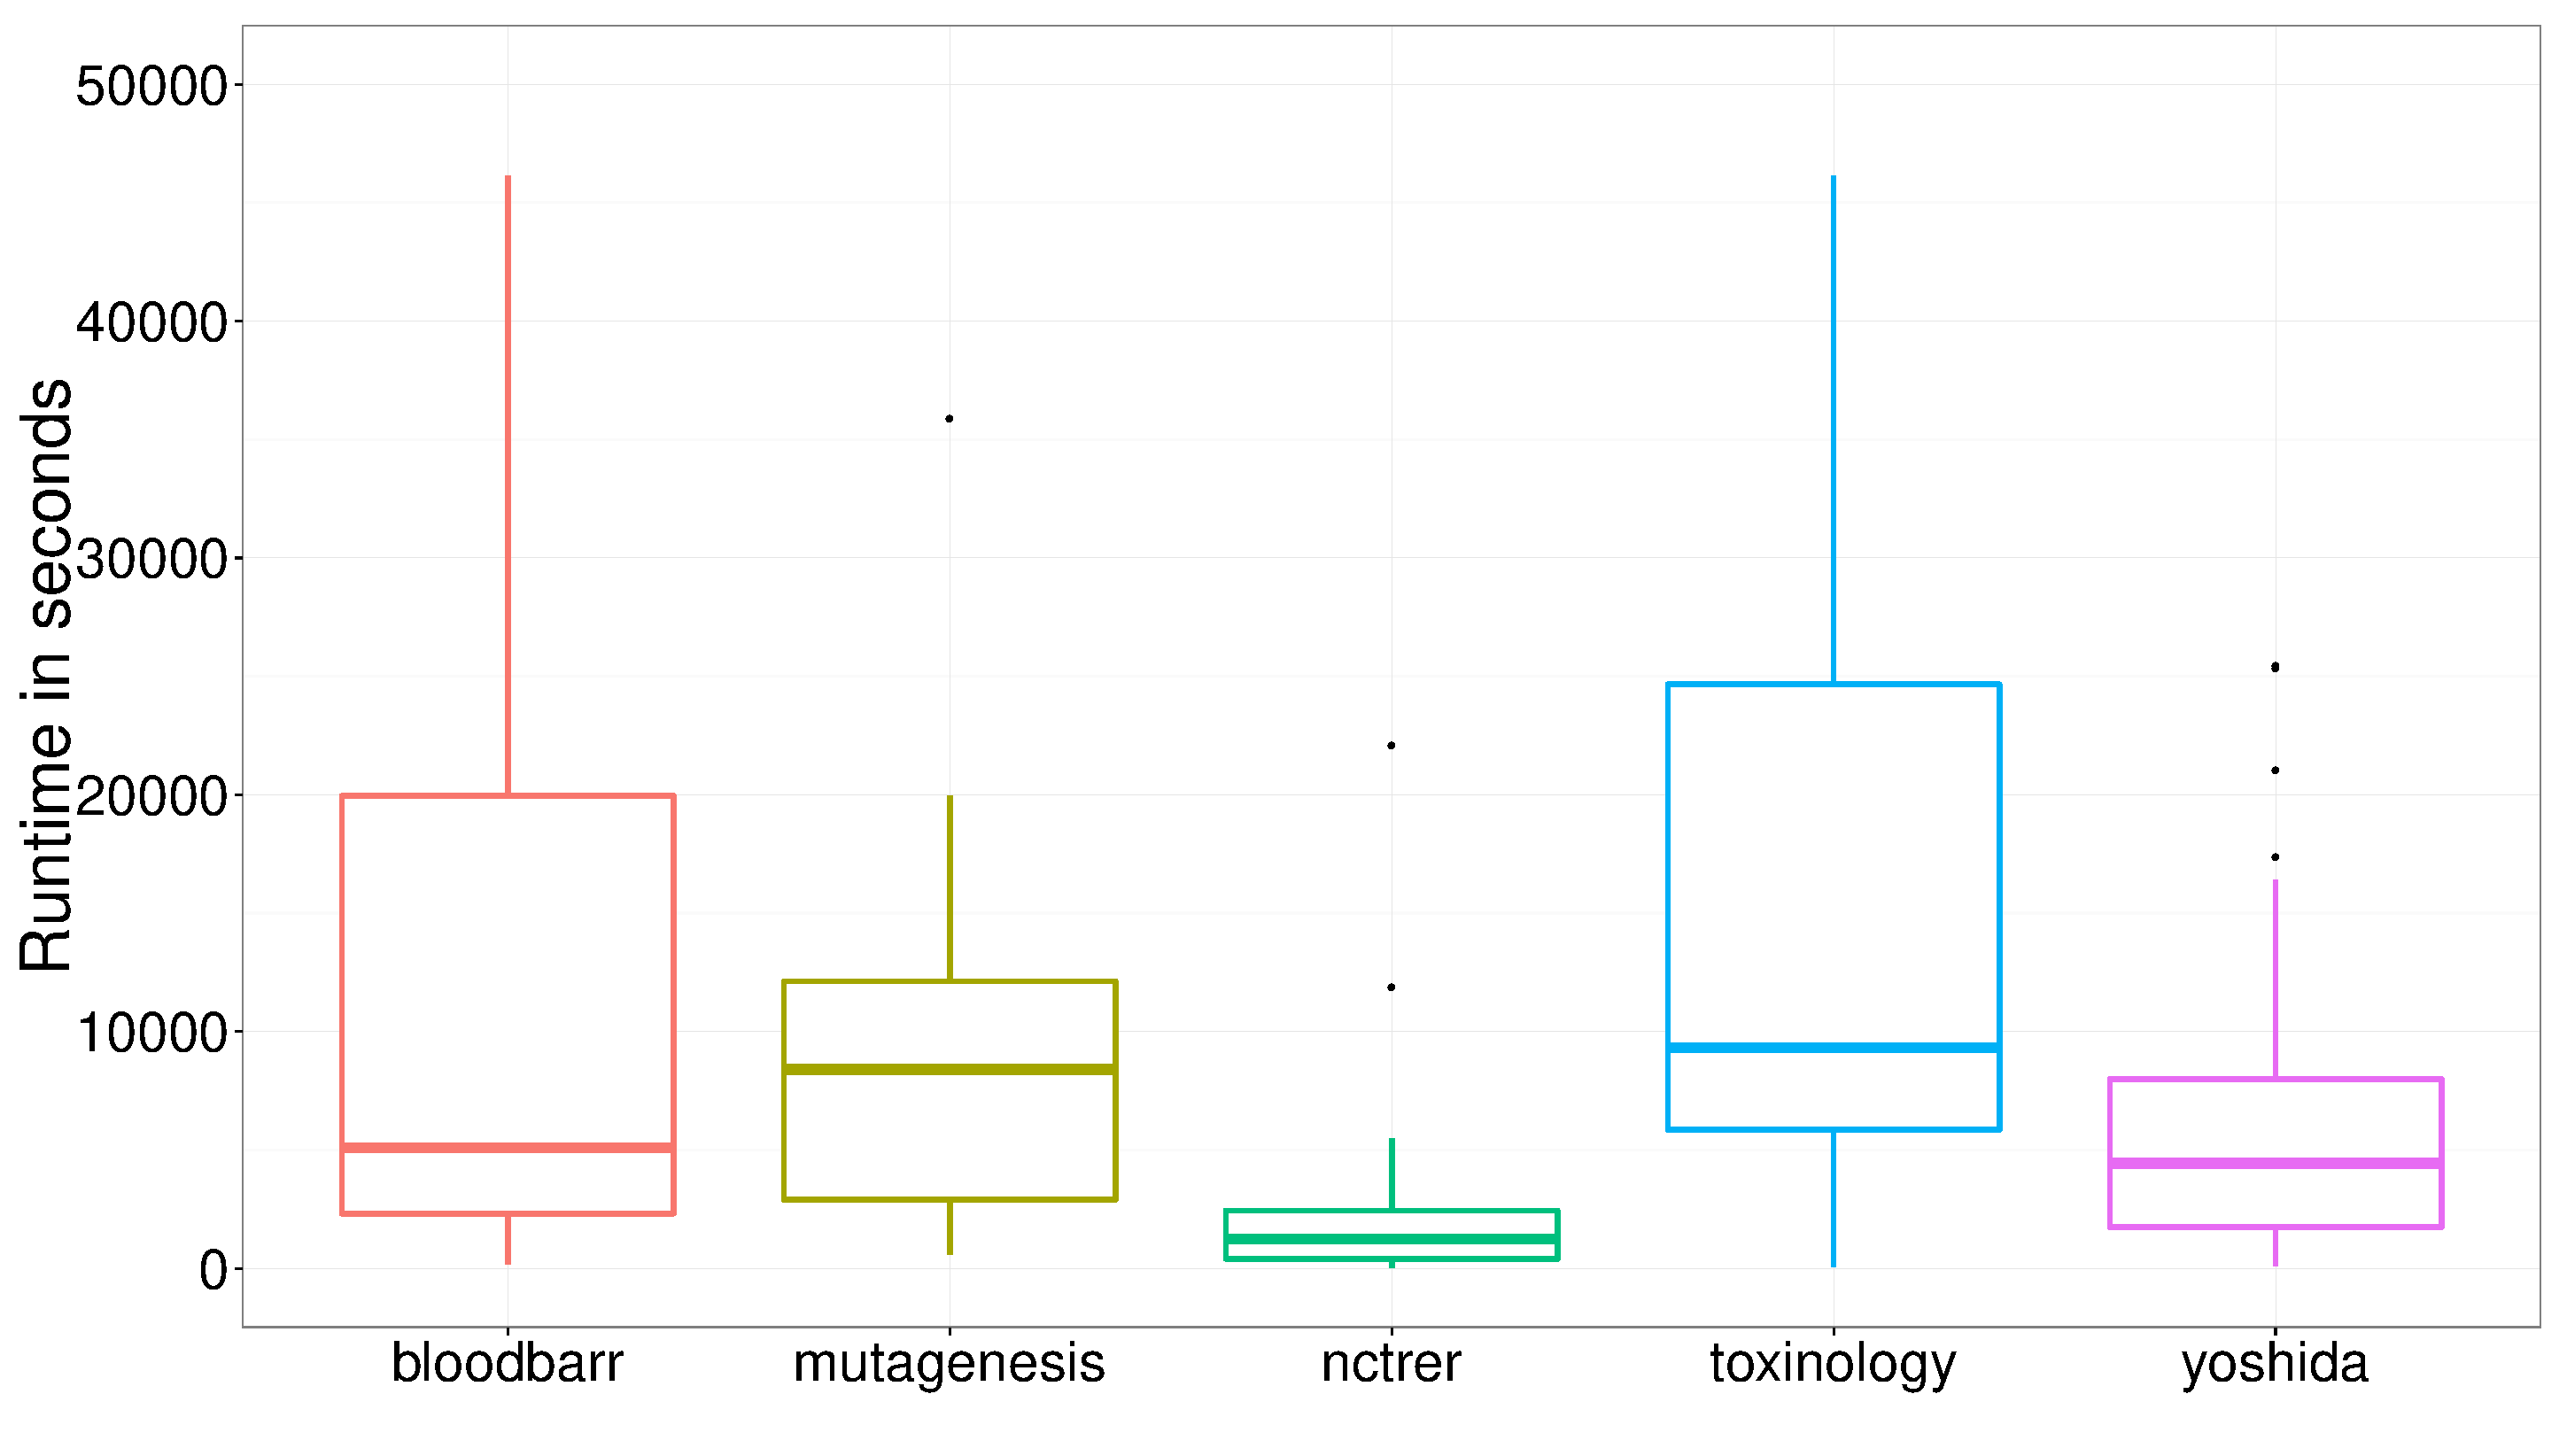
\includegraphics[width=1.06\linewidth]{figure_top_one_experiment.pdf}
      \caption{Top-$1$ runtime distribution \\(maximal patterns; first order model)}
      \label{fig:fol_top_experiments}
    \end{subfigure}
  \end{center}
  \captionsetup{
    font={small},
    skip={-10pt}
  }
  \caption{Dataset description and the summary of subsumption and top-$1$ experiments}
\end{figure}
In this section we evaluate the encoding on three problems: 1) classical $\theta$-subsumption performed by IDP as encoded in Eq. \ref{eq:full_subsumption}, 2) the first order model in Algorithm \ref{algo:top_cycle} on the frequent query mining task, and 3) the first order model on the top-$1$ query mining task. In all experiments the frequency threshold $t$ is set to $5\%$.
Since the task involves making a stochastic decision, i.e., \textit{pick-language-bias} in Algorithm \ref{algo:top_cycle} picks a graph from the dataset at random, this choice may significantly influence the running time. To resolve this issue, for the graph enumeration problem we average over multiple runs for each dataset: each run involves the enumeration of many queries, i.e., each run generates many data points (runtimes to enumerate $N$ queries). 
For the top-one mining problem, we present multiple runs for each dataset, since each run computes only one data point (runtime for the top-$1$ query). All experiments have been executed in a single thread on a 64-bit Ubuntu machine with Intel Core i5-3570 CPU @ 3.40GHz x 4 and 8GB memory.

\paragraph{Subsumption}
We evaluate how the IDP model \ref{eq:full_subsumption} encoding of $\theta$-subsumption compares with subsumption engine The Subsumer \parencite{subsumer}. We used the data from the original Subsumer experiments (transition phase on the subsumption hardness \cite[p. 327]{luc_book}) and evaluated IDP subsumption programs and Subsumer on a single hypothesis-example test, i.e., for each hypothesis and example we have made a separate call to IDP and Subsumer to establish subsumption.

The goal of this experiment is to compare how both systems perform if computations are done on a single example. We would like to estimate the potential gain in IDP, if we could specify a homomorphism existence check for each graph independently, like in a higher-order model Eq. \ref{eq:ho-matching}, i.e., for each graph we would check existence of some $\theta(X)$ instead of checking existence of one function $\theta(G,X)$ like in the first order model.

Figure \ref{figure:subsumption} indicates that IDP and Subsumer perform within a constant bound when we make a separate call for each example and hypothesis. That is, for all but one dataset, the runtimes are within the same order of magnitude for the two methods. If the internal structures of the system are reused and the call is made only for one hypothesis per \emph{set} of examples, we observe a speedup of at least one order of magnitude in Subsumer. This indicates that the system is able to efficiently use homomorphism independence. Once the solver community will have built extensions of systems like IDP to take advantage of homomorphism independence, the resulting systems will perform substantially better than the current ones and their performance will be close to that of special purpose systems such as Subsumer. More precisely, systems should exploit that it is computationally easier to find $n$ functions $\theta(X)$, than one $\theta(G,X)$ for $n$ values of $G$. 

\paragraph{Datasets and implementation}
We now evaluate the query mining models on a number of well-known and publicly available datasets: Blood Barrier, NCTRER and Yoshida datasets are taken from \parencite{featureset}, Mutagenesis and Enzymes datasets are from \parencite{mutagenesis_and_enzymes_datasets}, Toxinology dataset is from \parencite{toxinologydatatset}. A summary of the dataset properties is presented in Table \ref{table:datasets}. 

\paragraph{Top-$1$ performance evaluation}
We present the results of evaluating the FOL model for top-$1$ mining in Figure \ref{fig:fol_top_experiments}. Results were only obtained for the maximal size, and no solutions were computed for Enzymes in a reasonable time ($<$10h). The discriminative setting cannot be modeled and solved, since we need higher order primitives and for maximal coverage we already experienced an explosion of the search space. This experiment demonstrates that current satisfiability solvers cannot effectively perform search on both categories of query variables and homomorphism coverage; solver extensions are necessary. The first extension is to specify independence of the homomorphisms in the model, i.e., higher order primitives as indicated in the model Eq. \ref{eq:ho-matching}, the second is to give more control over the solver's decisions, e.g., by allowing to specify a decision order.

\paragraph{Frequent query mining}
The goal of the next experiment is to estimate the potential gain of the introduction of a higher order modeling construction. To do this, we mimicked the higher order behavior in Algorithm \ref{algo:top_cycle} by making several calls to IDP (one per graph) in the method \getquery. We call this mimicking model \textit{decomposed}. The results of the evaluation are presented in Figure \ref{table:query_enumeration}, a comparison of the decomposed and the original FOL model are in Figure \ref{fig:fol_enumeration_experiments}. Homomorphism dependence in the first order model causes serious computational difficulties, which makes higher order primitives one of the main priorities for solving query mining. The runtime also grows with the size of a pattern since it affects the search space and runtime as a result. %The canonicity check takes around $10^{-4}$ percent of the complete runtime.
\begin{figure}[thb]
  \captionsetup{
    skip=-0pt,
    font={small}
  }
  \begin{center}
    \begin{subfigure}{1\textwidth}
      \captionsetup{
        font={scriptsize},
        skip= 0pt
      }
      \scalebox{0.75}{
        \begin{tabular}{l l r r r r r}
          \textbf{dataset} & \textbf{model} & 1 & 5 & 10 & 25 & 50\\
          \hline

          \multirow{2}{*}{mutagenesis} & FOL  & 35s & 2m25s & 7m22s & 23m22s & 1h29m \\
          & \textbf{decomposed} & \textbf{17s} & \textbf{43s} & \textbf{84s} & \textbf{3m50s} & \textbf{9m26s} \\
          \multirow{2}{*}{nctrer}      & FOL  & 30s & 3m24s & 7m17s & 24m28s & 1h27m \\
          & \textbf{decomposed }& \textbf{5s} & \textbf{35s} & \textbf{1m16s} & \textbf{6m0s}&  \textbf{9m20s}\\
          \multirow{2}{*}{yoshida}     & FOL  & 35s & 2m53s & 6m34s & 31m13s & 1h56m \\
          & \textbf{decomposed} & \textbf{9s} & \textbf{1m1s} & \textbf{2m0s} & \textbf{5m48s} & \textbf{15m8s} \\
          \multirow{2}{*}{bloodbarr}   & FOL  & 1m4s & 6m26s & 15m51s & 1h47m & 8h2m \\
          & \textbf{decomposed}  & \textbf{9s} & \textbf{57s} & \textbf{2m3s} & \textbf{9m55s} & \textbf{14m52s} \\
          \multirow{2}{*}{toxinology}  & FOL  & 1m21s & 8m20s & 22m5s & 2h42m  & 16h3m\\
          & \textbf{decomposed} & \textbf{11s} & \textbf{56s} & \textbf{2m35s} & \textbf{7m54s} &  \textbf{18m5s}\\
          \multirow{2}{*}{enzymes}     & FOL  & 7m3s & 45m48s & 4h0m & ---- & ----- \\
          & \textbf{decomposed} & \textbf{15s} & \textbf{1m27s} & \textbf{2m57s} & \textbf{13m26s} & \textbf{38m16s}\\

        \end{tabular}}
        \vspace{3pt}
        \caption{Frequent query enumeration time of $N$ queries}
        \label{table:query_enumeration}
      \end{subfigure}
      \hfill 
      \begin{subfigure}{1\textwidth}
        \captionsetup{
          font={scriptsize},
          skip=-0pt
        }
        \phantom{text}
        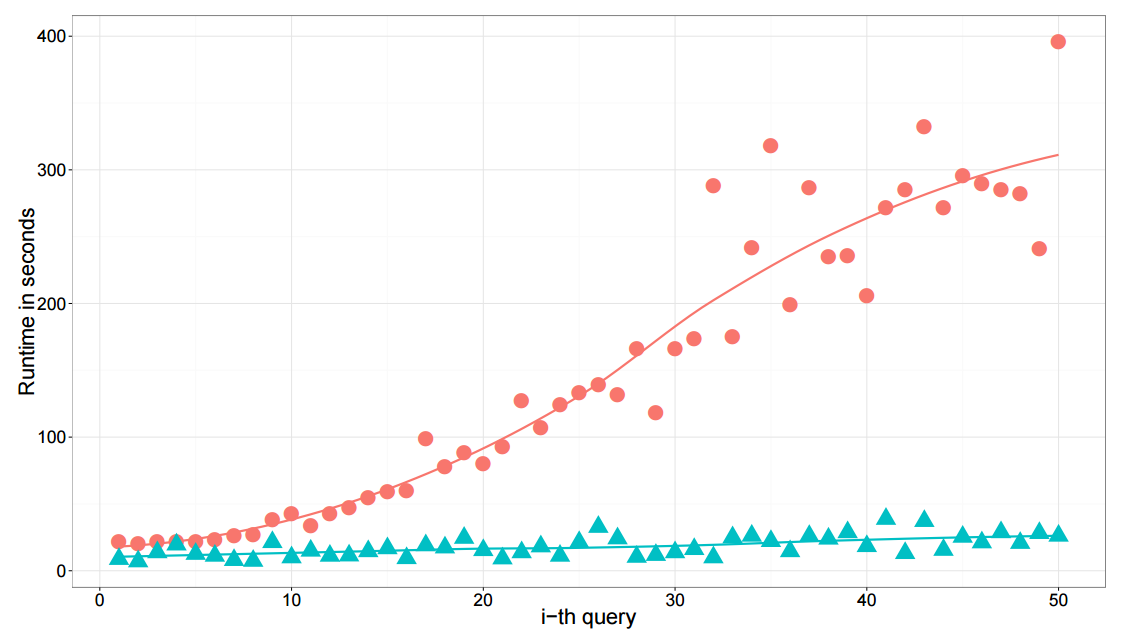
\includegraphics[width=1.00\linewidth]{figure_runtime_decomposition.png}
        \caption{Runtime of $i$-th query (in s; y-axis) on yoshida dataset\\(x-axis is the query index $i$)}
        \label{fig:fol_enumeration_experiments}
      \end{subfigure}
    \end{center}
    \captionsetup{
      font={small},
      skip=-10pt
    }
    \caption{Frequent query enumeration FOL (blue) vs decomposed model (red)}
  \end{figure}

\paragraph{Summary of the experimental results}
The results show that the model performs reasonably and we therefore conclude that it can be considered a first step towards the development of declarative languages for relational query mining. From Figure \ref{figure:subsumption} and \ref{table:query_enumeration} it is clear that the core computational difficulty lies in the inability to state homomorphism independence. 
This follows from the candidate generation and canonicity check runtime and from the speedup that Subsumer has when it is applied to the whole set of examples with one call. After comparing the performance of  IDP and Subsumer on a single example and observing the speed up of the decomposed model in Figure \ref{table:query_enumeration}, one would expect a significant speedup if it were implemented within the solver.

  We have observed in Figure \ref{fig:fol_top_experiments} that query mining introduces interesting computational challenges and might be of interest to the solver development community as well as to the ILP community. We also pointed out the reasons for these computational difficulties and suggested possible ways to enhance the solvers.

\section{Model discussion and generalization}
\label{sec:approach_extension}
\paragraph{Advantages and disadvantages of the model}
There is a number of advantages of the declarative approach to pattern mining as compared to the classical imperative methods: compact and clear representation; extendability and generality; provability and formal semantics of the models; reliable and portable implementation (the solvers developed by the community, well tested and already applied to a variety of tasks; the solvers are available for all popular operation systems: Linux, MacOS and Windows).

In particular, our model represents compactly not only the model of graph mining problem but also the code that can be executed to solve the problem. Adding the source code of gSpan \parencite{gspan} to a paper ($\sim2000$ lines of C++) would be impossible. Also the model can be easily extended by adding constraints to the theory, e.g. adding a constraint to handle labels on edges is just an extra line with a straightforward logical formula. The last but not least our formulation allows formal rigorous reasoning on the constraints that constitute the model.

These advantages come, of course, not without a cost. Typically, specialized algorithms perform an order of magnitude (at least) faster. The main reason for such a speed up is the heuristic approach incorporated in most of the mining algorithms that takes advantage of the structure of the problem. Our experiments in Figure \ref{fig:fol_enumeration_experiments} demonstrate that the declarative approach can reduce the runtime gap by extending the language to better incorporate the structure of a problem. Also, modeling this kind of mining tasks influences the way declarative solvers are built and potentially can lead to better solving systems that would perform reasonable on mining takes.
\paragraph{Generalization of the approach}
Let us demonstrate how the model can be extended to handle labels on the edges as an example how declarative systems can be adapted to solve new tasks.

Assume that the edge labels are represented using the predicate $\edgelabel(g,e_1,e_2,l)$ and the edge labels of the bottom clause are stored in the predicate  $\tedgelabel(e_1,e_2,l)$. Then, the first order formulation Eq. \ref{constr:fol_matching} can be extended by adding the constraint:
\begin{equation*}
\invar(X) \wedge \invar(Y) \wedge \tedgelabel(X,Y,L) \implies \edgelabel(G,\theta(G,X), \theta(G,Y), L).
\end{equation*}
Intuitively, this constraint ensures that if there is an edge $(X,Y)$ with a label $L$ in the bottom clause, then there is an edge with a l label $L$ in the graph $G$. If each edge has a label, the constraint above can replace the first constraint in Eq. \ref{constr:fol_matching}.

The smallest change, according to the principle, is the addition of a rule or a fact.n general this example demonstrates how declarative approach and our model in particular implements the elaboration tolerance principle \parencite{elaboration_tolerance}, i.e. a small change in the problem formulation, should introduce a small change in the model. The smallest changes, according to the principle, is the addition of a rule or a fact. With this respect our model satisfies elaboration tolerance principle and can be called an additive elaboration.
\section{Related work} \label{sec:related_work}
WARMR \parencite{warmr} and FARMER \parencite{farmer} are extensions of the Apriori algorithm for discovering frequent structures in multiple relations. Even though they use ILP techniques (e.g., a declarative language bias) to determine frequent queries, they imperatively specify computations and the algorithms do not support the addition of arbitrary constraints due to the restricted nature of the algorithm, and hence focus on a more specific task. C-Farmr \parencite{condensed_luc} is an ILP system for frequent Datalog clauses that uses so-called condensed representations to avoid the generation of semantically equivalent clauses. %Aleph \parencite{aleph} is an extension of Prolog language to learn horn clauses. It can be used to program discovery of rules in the relational data using mode declarations and background knowledge.

The XHAIL system \parencite{xhail} uses ASP as a computational engine to perform abductive inductive reasoning. It is similar in the way we use an ASP engine as computational core, but XHAIL focuses on the abduction task, whereas we focus on query mining which always involves aggregation and model enumeration.

In the work on sequence testing \parencite{asp_sequence_testing} ASP is used as a subroutine in a cycle and model projection on a predicate is also present similarly to our Algorithm \ref{algo:top_cycle}, but this similarity is technical, since the tasks are of a different nature. ASP has also been applied to itemset mining \parencite{asp_itemset} and sequence mining \parencite{seq_asp}, but these methods only deal with one particular task in its basic formulation. 

gSpan \parencite{gspan} and B-AGM, Biased-Apriori-based Graph Mining \parencite{bagm}, are specialized algorithm designed to solve the frequent graph pattern mining problem. The algorithm is tailored to solve only one task exclusively and requires significant changes in its core to be extended to solve other mining tasks (and, to the best of our knowledge, there is no extension to the full relation setting). It is similar, however, in the computational challenges: canonicity checks, homomorphism checks, language bias etc. 
\section{Conclusions}\label{sec:conclusions}
We have shown that modern ASP solvers, in principle, can be applied to ILP query mining tasks. We have provided experimental evidence that these models can be used as prototypes for developing declarative mining languages. We have also indicated the reasons why the solvers could be extended to make computation efficient and proposed concrete extensions as well as estimated their potential effectiveness. The query mining models and the experimental setup we developed provide an interesting challenge for the ASP community and a potentially useful tool for the ILP community.




\section{Hybrid ASP-based Approach to Pattern Mining}

  Detecting small sets of relevant patterns from a given dataset is a central challenge in data mining. The relevance of a pattern is based on user-provided criteria; typically, all patterns that satisfy certain criteria are considered relevant. Rule-based languages like Answer Set Programming (ASP) seem well-suited for specifying such criteria in a form of constraints.  Although progress has been made, on the one hand, on solving individual mining problems and, on the other hand, developing generic mining systems, the existing methods either focus on scalability or on generality.  In this chapter we make steps towards combining local (frequency, size, cost) and global (various condensed representations like maximal, closed, skyline) constraints in a generic and efficient way. We present a hybrid approach for itemset and sequence mining which exploits dedicated highly optimized mining systems to detect frequent patterns and then filters the results using declarative ASP. Experiments on real-world datasets show the effectiveness of the proposed method and computational gains both for itemset and sequence mining. 
 
\section{Introduction to Hybrid Approach}
\paragraph{Motivation} 
Availability of vast amounts of data from different domains has led to an increasing interest in the development of scalable and flexible methods for data analysis.
A key feature of flexible data analysis methods is their ability to incorporate users' background knowledge and different criteria of interest. They are often provided in the form of \emph{constraints} to the valid set of answers, the most common of which is the frequency threshold: a pattern is only considered interesting if it appears often enough. Mining all frequent (and otherwise interesting) patterns is a very general problem in data analysis, with applications in medical treatments, customer shopping sequences, Weblog click streams and text analysis, to name but a few examples.

Most data analysis methods consider only one (or few) types of constraints, limiting their applicability. Constraint Programming (CP) has been proposed as a general approach for (sequential) mining of frequent patterns~\parencite{DBLP:books/mit/fayyadPSU96/AgrawalMSTV96}, and Answer Set Programming (ASP) \parencite{GL1988} has been proved to be well-suited for defining the constraints conveniently thanks to its expressive and intuitive modelling language and the availability of optimized ASP solvers (see e.g., \parencite{DBLP:conf/lpnmr/Jarvisalo11,DBLP:conf/ijcai/GebserGQ0S16,DBLP:journals/corr/GuyetMQ14} for existing approaches). 


In general, all constraints can be classified into \emph{local constraints}, that can be validated by the pattern candidate alone, and \emph{global constraints}, that can only be validated via an exhaustive comparison of the pattern candidate against all other candidates. Combining local and global constraints in a generic way is an important and challenging problem, which has been widely acknowledged in the constraint-based mining community.  Although progress has been made, on the one hand, on solving individual mining problems and, on the other hand, on developing generic mining systems, the existing methods either focus on scalability or on generality, but rarely address both of these aspects. This naturally limits the practical applicability of the existing approaches.

\paragraph{State of the art and its limitations} Purely declarative ASP encodings for frequent and maximal itemset mining were proposed in \parencite{DBLP:conf/lpnmr/Jarvisalo11}. In this approach, first every item's inclusion into the candidate itemset is guessed, and the guessed candidate pattern is checked against frequency and maximality constraints. While natural, this encoding is not  truly generic, as adding extra local constraints requires significant changes in it. Indeed, for a database, where all available items form a frequent (and hence maximal) itemset, the maximal ASP encoding has a single model. The latter is, however, eliminated once restriction on the length of allowed itemsets is added to the program. This is undesired, as being maximal
is not a  property of an itemset on its own, but rather %its property %of an itemset 
in the context of a collection of other itemsets \parencite{DBLP:journals/kais/BonchiL06}. Thus, ideally one would be willing to first apply all local constraints and only afterwards construct a condensed representation of them, which is not possible in \parencite{DBLP:conf/lpnmr/Jarvisalo11}. % Moreover, the implementation \parencite{ }, the subset inclusion relation thus needs to be checked exponential number of times.

This shortcoming has been addressed in the recent work \parencite{DBLP:conf/ijcai/GebserGQ0S16} on ASP-based sequential pattern mining, which exploits ASP preference-handling capacities to extract patterns of interest and supports the combination of local and global constraints. However, both \parencite{DBLP:conf/ijcai/GebserGQ0S16} and \parencite{DBLP:conf/lpnmr/Jarvisalo11} present %exploits a 
purely declarative encodings, which suffer from scalability issues caused by the exhaustive exploration of the huge search space of candidate patterns. The subsequence check amounts to testing whether an embedding exists (matching of the individual symbols) between sequences. In sequence mining, a pattern of size $m$ can be embedded into a sequence of size $n$ in $O(n^m)$ different ways, therefore, clearly a direct pattern enumeration is unfeasible in practice. 

While a number of individual methods tackling selective constraint-based mining tasks exist (see Tab.~\ref{tab:comparison} for comparison) there is no uniform ASP-based framework that is capable of effectively combining constraints both on the global and local level and is suitable for itemsets and sequences alike.

\paragraph{Contributions} The goal of our work is to make steps towards building a generic framework that supports  mining of condensed (sequential) patterns, which (1) effectively combines dedicated algorithms and declarative means for pattern mining and (2) is easily extendable to incorporation of various constraints. More specifically, the salient contributions of our work can be summarized as follows:

\begin{itemize}
  \item  We present a general extensible pattern mining framework for mining patterns of different types using ASP.
  \item  We introduce a feature comparison, such as closedness under solutions, between different ASP mining models and dominance programming, which is a generic itemset mining language and solver.
  \item  We demonstrate the feasibility of our approach with an experimental evaluation across multiple itemset and sequence datasets.
\end{itemize}

%\paragraph{Structure} 
%After providing necessary background in Sec.~\ref{sec:prelim} we introduce our approach in Sec.~\ref{sec:appr}, describe experimen al results in Sec.~\ref{sec:eval} and conclude the paper with related work discussion and final remarks in Sec.~\ref{sec:relwork} and Sec.~\ref{sec:concl} respectively.

\begin{table}[t]
  \centering
 
  \vspace{15pt}
  \setlength\tabcolsep{3.0pt}
  \begin{tabular}{|l | c | c | c | c | c|}
\hline
    \textbf{Datatype}                & \textbf{Task}                  & \rotatetxt{\cite{DBLP:conf/lpnmr/Jarvisalo11}} & \rotatetxt{\cite{DBLP:conf/ijcai/GebserGQ0S16}} & \rotatetxt{\cite{dp2013}} &  \rotatetxt{\textbf{Our work}} \\  \hline  \hline
                                                                                                                                                                      
  \multirow{3}{*}{\textbf{Itemset}}  & frequent pattern mining        &  \checkmark      &  \na        & \checkmark       & \checkmark   \\ 
                                     & condensed (closed, max, etc)   & $\checkmark^{*}$ &  \na        & \checkmark       & \checkmark   \\ 
                                     & condensed under constraints    &  \na             &  \na        & \checkmark       & \checkmark   \\\hline    
  \multirow{3}{*}{\textbf{Sequence}} & frequent pattern mining        &  \na             & \checkmark  & \na              & \checkmark   \\ 
                                     & condensed (closed, max, etc)   &  \na             & \checkmark  & \na              & \checkmark   \\ 
                                     & condensed under constraints    &  \na             & \checkmark  & \na              & \checkmark       \\
\hline                                                                                                                                              
  \end{tabular} 
\smallskip

 \caption{Feature comparison between various ASP mining models and dominance programming (``\na'' : ``not designed for this datatype'', $\checkmark^*$ : only maximal is supported)}
  \label{tab:comparison}
\end{table}

\section{Hybrid ASP-based Mining Approach}\label{sec:problem}

% The goal of this work is to allow for hybradisation between highly optimized generic solvers and specialized pattern mining implementations within a generic framework for pattern mining under both local and global constraints.
In this section we present our hybrid method for frequent pattern mining. Unlike previous ASP-based mining methods, our approach combines highly optimized algorithms for frequent pattern discovery with the declarative ASP means for their convenient post-processing. Here, we focus on itemset and sequence mining; however our approach can be also applied to subgraph discovery (details are left for future work). 

Given a frequency threshold $\sigma$, a (sequential) dataset $D$ and a set of constraints $\cC=\cC_l\cup\cC_g$, where $\cC_l$ and $\cC_g$ are respectively local and global constraints, we proceed in two steps as follows. 
\bigskip

\paragraph{Step 1} First, we launch a dedicated optimized algorithm to extract all (sequential) frequent patterns from a given dataset, satisfying the minimal frequency threshold $\sigma$. Here, any frequent pattern mining algorithm can be invoked. %, the ones 
We use Eclat \parencite{eclat} for itemsets and PPIC \parencite{PPIC} for sequences.
\bigskip

\paragraph{Step 2} Second, the computed patterns are post-processed using the declarative means to select a set of \emph{valid} patterns (i.e., those satisfying constraints in $\cC_l$). For that the frequent patterns obtained in Step 1 are encoded as facts \texttt{item(i,j)} for itemsets and \texttt{seq(i,j,p)} for sequences where \texttt{i} is the pattern's ID, \texttt{j} is an item contained in it and \texttt{p} is its position. The local constraints in $\cC_l$ are represented as ASP rules, which collect IDs of patterns satisfying constraints from $\cC_l$ into the dedicated predicate \texttt{valid}, while the rest of the IDs are put into the \texttt{not\_valid} predicate. 

Finally, from all valid patterns a desired condensed representation is constructed by storing patterns \texttt{i} in the \texttt{selected} predicate if they are not \texttt{dominated} by other valid patterns based on constraints from $\cC_g$. Following the principle of \parencite{DBLP:conf/lpnmr/Jarvisalo11}, in our work every answer set represents a single desired pattern, which satisfies both local and global constraints. The set of all such patterns forms a condensed representation. In what follows we discuss our encodings of local and global constraints in details. 



\subsection{Encoding Local Constraints} 

In our declarative program we specify local constraints by the predicate \texttt{valid}, which reflects the conditions given in Def.~\ref{def:val}. For every constraint in $\cC_l$ we have a set of dedicated rules, stating when a pattern is not valid. 
For instance, a constraint checking whether the cost of items in a pattern exceeds a given threshold $N$ is encoded as % using the following rule:
%\sergey{we, actually have size precomputed for each pattern from the wrapper and/or the specialized algo, so cost here}

\small{\begin{center}
\texttt{not\_valid(I) :- \#sum\{C:item(I,J),cost(J,C)\} > N, pattern(I).}
\end{center}}

\normalsize{A similar rule for sequences can be defined as follows: }% obtained by substituting \texttt{item(I,J)} with \texttt{seq(I,J,P)}. Taking into account repeated items would result in a rule

\small{\begin{center}
\texttt{not\_valid(I) :- \#sum\{C:seq(I,J,P),cost(J,C)\} > N, pattern(I).}
\end{center}}

 
% Provided that every item in a set has some weight assigned to it we could generalize the above rules to obtain constraints restricting the allowed weight in a pattern.
\normalsize{Analogously, one can specify arbitrary domain constraints on patterns. }

\begin{example}
Consider a dataset storing moving habits of young people during their studies. Let the dedicated frequent sequence mining algorithm return the following patterns: $S_1=\mi{\tuple{bG\,mF\,ba\,mG\,ma}}$; $S_2=\mi{\tuple{bF\,mG\,ba\,mF\,ma}}$; $S_3=\mi{\tuple{bA\,ba\,ma}}$, where $\mi{bG,}$\\$\mi{bF,bA}$ stand for born in Germany, France and America, $\mi{ba,ma}$ stand for bachelors and masters and the predicates $\mi{mG,mF}$ reflect that a person moved to Germany and France, respectively. Suppose, we are only interested in moving habits of Europeans, who got their masters degree from a German university. The local domain constraint expressing this would state that (1) $\mi{bA}$ should not be in the pattern, while (2) either both $\mi{bG}$ and $\mi{ma}$ should be in it without any $\mi{mF}$ in between or $\mi{mG}$ should precede $\mi{ma}$. These constraints are encoded in the program in List.~\ref{ex:move}. From the answer set of this program we get that both  $S_2$ and $S_3$ are not valid, while $S_1$ is. \qed

 \begin{figure}[t]
 \small{
 \begin{lstlisting}[language=ASPlang,label=ex:move,caption=Moving habits of people during studies, escapeinside={@}{@}]
time(1..5).
@\commenttextasp{\% people born in Germany or France are Europeans}@
eu(I) :- seq(I,bG,P).
eu(I) :- seq(I,bF,P).
@\commenttextasp{\% collect those who moved to France before P}@
moved_before(X,P) :- seq(X,mF,P1), P>P1, time(P), time(P1).
@\commenttextasp{\% collect those who moved to France after P and before masters}@
moved_after(X,P) :- seq(X,mF,P1), seq(X,ma,P2), P<P1, 
                    p1<P2, time(P), time(P1), time(P2).
@\commenttextasp{\% keep Europeans who moved to Germany straight before masters}@
keep(X) :- seq(X,ma,P+1), seq(X,mG,P), eu(X).
@\commenttextasp{\% keep Germans who did not move before masters}@
keep(X) :- seq(X,bG,P1), seq(X,ma,P), not moved_before(X,P).
@\commenttextasp{\% keep Europeans whose last move before masters was to Germany}@
keep(X) :- seq(X,mG,P1), seq(X,ma,P2), P1<P2,  
           eu(X), not moved_after(X,P1).
@\commenttextasp{\% a pattern is not valid, if it should not be kept}@
not_valid(X) :- pattern(X), not keep(X)
 \end{lstlisting}
}
 \end{figure}
\end{example}



% \begin{figure}[t]
% %\begin{lstlisting}[language=ASPlang,firstnumber=1,label=ex:move,caption=Moving habits of people during studies escapeinside={@}{@}]
% \small{
% \begin{lstlisting}[language=ASPlang,label=ex:move,caption=Moving habits of people during studies, escapeinside={@}{@}]
% @\commenttextasp{\% people born in Germany or France are Europeans}@
% seq(I,e,P) :- seq(I,bG,P)
% seq(I,e,P) :- seq(I,bF,P)
% @\commenttextasp{\% collect moving actions regardless of a European destination}@
% seq(I,m,P) :- seq(I,mG,P)
% seq(I,m,P) :- seq(I,mF,P)
% @\commenttextasp{\% keep Europeans who moved to Germany straight before masters}@
% keep(X) :- pattern(X), seq(X,ma,P'+1), seq(X,mG,P'), seq(X,e,P)
% @\commenttextasp{\% collect people who moved somewhere before time point P}@
% moved_before(X,P) :- pattern(X), seq(X,m,P'), P>P'
% @\commenttextasp{\% collect people who moved somewhere after time point P and before masters}@
% moved_after(X,P) :- pattern(X), seq(X,m,P'), P<P', 
%                     P'<P'', seq(X,ma,P'')
% @\commenttextasp{\% keep Germans who did not move before masters}@
% keep(X) :- pattern(X), seq(X,bG,P'), seq(X,ma,P), 
%            not moved_before(X,P)
% @\commenttextasp{\% keep Europeans whose last move before masters was to Germany}@
% keep(X) :- pattern(X), seq(X,e,P'), seq(X,ma,P), 
%            seq(X,mG,P''), P''<P, not moved_after(X,m,P'')
% @\commenttextasp{\% a pattern is not valid, if it should not be kept}@
% \end{lstlisting}}
% \end{figure}

%@\commenttextasp{\% keep patterns about Europeans who finished masters in Germany}@

\normalsize{
To combine all local constraints from $\cC_l$ we add to a program a generic rule specifying that a pattern \texttt{I} is valid whenever \texttt{not\_valid(I)} cannot be inferred. }

\small{
\begin{center}
\texttt{valid(I) :- pattern(I), not not\_valid(I)}
\end{center}}

\normalsize{Patterns \texttt{i}, for which \texttt{valid(i)} is deduced are then further analyzed to construct a condensed representation based on global constraints from $\cC_g$.}
% Intuitively, for that we come up with a respective ASP encoding. For every condensed representation we present its dedicated encoding both for itemsets are sequences. 


\subsection{Encoding Global Constraints}

The key for encoding global constraints is the declarative formalization of the dominance relation (Def.~\ref{def:dom}). For example, for itemsets the maximality constraint boils down to pairwise checking of subset inclusion between patterns. For sequences this requires a check of embedding existence between sequences.



 Regardless of a pattern type from $\cL$ %and a global constraint from 
and a constraint from $\cC_g$ every encoding presented 
in this section is supplied with a rule, which guesses (\texttt{selected/1} predicate) a single \texttt{valid} pattern to be a candidate for inclusion in the condensed representation, and a constraint that rules out \texttt{dominated} patterns thus enforcing a different guess. 
% guesses a candidate pattern () among all valid patterns.


\small{\begin{center}
\texttt{1 \{selected(I) : valid(I)\} 1.}
\end{center}

\begin{center}
\texttt{ :- dominated.}
\end{center}}

% The encoding of conditions %rules 
% specific for a %every 
% pattern type and a constraint stating when %then encode conditions stating when %the 
%  \texttt{dominated/0} is derived .

 \begin{figure}[t]
\small{
 \begin{lstlisting}[language=ASPlang,label=lst:max,caption=Maximal itemsets encoding, escapeinside={@}{@}]
@\commenttextasp{\% I is not a subset of J if I has items that are not in J}@
not_subset(J) :- selected(I), item(I,V), not item(J,V), 
                 valid(J), I != J.
@\commenttextasp{\% derive dominated whenever I is subset of J}@
dominated :- selected(I), valid(J), 
             I != J, not not_subset(J).
\end{lstlisting}}
 \end{figure}
 \normalsize{In what follows, we discuss concrete realizations of the dominance relation both for itemsets and sequences for various global constraints, i.e., we present specific rules related to the derivation of the \texttt{dominated/0} predicate.
}

\paragraph{Itemset Mining} We first provide an encoding for maximal itemset mining in List~\ref{lst:max}. To recall, a pattern is \emph{maximal} if none of its supersets is frequent. An itemset $I$ is included in $J$ iff for every item $i\in I$ we have  $i\in J$. We encode the violation of this condition in lines (1)--(3). The second rule presents the dominance criteria.

For closed itemset mining a simple modification of List.~\ref{lst:max} is required. An itemset is \emph{closed} if none of its supersets has the same support. Thus to both of the rules from List.~\ref{lst:max} we need to add atoms \texttt{support(I,X), support(J,X)}, which store the support sets of \texttt{I} and \texttt{J} respectively (extracted from the output of Step 1).  

% \begin{lstlisting}[language=ASPlang,firstnumber=7,label=lst:cl,escapeinside={@}{@}]
% dominated :- selected(I), valid(J), support(I,X),
%              I != J, not not_subset(J), support(J,X).
% \end{lstlisting}
% \medskip

For free itemset mining the rules of the maximal encoding are changed as follows:
\medskip

\small{\begin{lstlisting}[language=ASPlang,firstnumber=4,label=lst:free,escapeinside={@}{@}]
not_superset(J) :- selected(I), item(J,V), not item(I,V), 
                   valid(J), I != J.
dominated :- selected(I), valid(J), support(I,X),
             I != J, not not_superset(J), support(J,X).
\end{lstlisting}}



\begin{figure}[t]
\small{\begin{lstlisting}[language=ASPlang,label=lst:sky,caption=Skyline itemsets encoding, escapeinside={@}{@}]
@\commenttextasp{\% support and size comparison among patterns}@
g_size_geq_fr(J) :- selected(I), valid(J), support(I,X), 
                    support(J,Y), size(I,Si), size(J, Sj), 
                    Si <  Sj, X <= Y. 
geq_size_g_fr(J) :- selected(I), valid(J), support(I,X), 
                    support(J,Y), size(I,Si), size(J, Sj), 
                    Si <= Sj, X < Y. 
@\commenttextasp{\% derivation of the domination condition}@
dominated :- valid(J), g_size_geq_fr(J). 
dominated :- valid(J), geq_size_g_fr(J). 
\end{lstlisting}}
\end{figure}
\normalsize{Finally, the skyline itemset/sequence encoding is given in List.~\ref{lst:sky}, where the first two rules specify the conditions (a) and (b) for skyline itemsets as specified in Sec.~\ref{sec:prelim}. }

\begin{figure}[t]
\small{ \begin{lstlisting}[language=ASPlang,label=lst:maxs,caption=Maximal sequence encoding, escapeinside={@}{@}]
@\commenttextasp{\% if V appears in a valid pattern I, derive in(V,I)}@
in(V,I) :- seq(I,V,P), valid(I).
@\commenttextasp{\% I is not a subset of J if I has V that J does not have}@
not_subset(J) :- selected(I), valid(J), I != J, 
                 seq(I,V,P), not in(V,J).
@\commenttextasp{\% if for a subseq <V,W> in I there is V followed}@
@\commenttextasp{\% by W in J then deduce domcand(V,J)}@
domcand(V,J,P) :- selected(I), seq(I,V,P), seq(I,W,P+1), I != J
                  valid(J), seq(J,V,Q), seq(J,W,Q'), Q'>Q.
@\commenttextasp{\% if domcand(V,J) does not hold for some V in I}@ 
@\commenttextasp{\% and a pattern J then derive not\_dominated\_by(J)}@
not_dominated_by(J) :- selected(I), seq(I,V,P), seq(I,W,P+1), 
                       I != J, valid(J), not domcand(V,P,J).
@\commenttextasp{\% if neither not\_dominated\_by(J) nor not\_subset\_of(J)}@
@\commenttextasp{\% are derived for some J, then I is dominated}@
dominated :- selected(I), valid(J), I != J, 
             not not_subset_of(J), not not_dominated_by(J). \end{lstlisting}}
 \end{figure}


\normalsize{\paragraph{Sequence Mining} 
The subpattern relation for sequences is slightly more involved, than for itemsets, as it preserves the order of elements in a pattern. To recall, a sequence $S$ is included in $S'$ iff an embedding $e$ exists, such that $S \sqsubseteq_e S'$.}

In List.~\ref{lst:maxs} we present the encoding for maximal sequence mining. A selected pattern is not maximal if it has at least one valid superpattern. We rule out patterns that are for sure not superpatterns of a selected sequence. First, obviously \texttt{J} is not a superpattern of \texttt{I} if \texttt{I} is not a subset of \texttt{J} (lines (4)--(5)), i.e., if \texttt{not\_subset(J)} is derived, then \texttt{J} does not dominate \texttt{I}. If \texttt{J} is a superset of \texttt{I} then to ensure that \texttt{I} is not dominated by \texttt{J}, the embedding existence has to be checked (lines (6)--(9)). \texttt{I} is not dominated by \texttt{J} if an item exists in \texttt{I}, which together with its sequential neighbor cannot be embedded in \texttt{J}.  This condition is checked in lines (10)--(13), where \texttt{domcand(V,J,P)} is derived if for an item \texttt{V} at position \texttt{P} and its follower, embedding in \texttt{J} can be found. 

The encoding for closed sequence mining is obtained from the maximal sequence encoding analogously as it is done for itemsets. The rules for free sequence mining are constructed by substituting lines (4)--(13) of List.~\ref{lst:maxs} with the following ones:


\small{\begin{lstlisting}[language=ASPlang,firstnumber=4,label=lst:free,escapeinside={@}{@}]
not_superset(J) :- selected(I), in(V,J), 
                   not in(V,I), I != J.
domcand(V,J) :- selected(I), seq(J,V,P), item(J,P+1,W), 
                item(I,V,Q), seq(I,W,Q'),Q'>Q, I != J.
not_dominated_by(J) :- selected(I), valid(J), I != J, 
                       seq(J,V,P), seq(J,W,P+1), 
                       not domcand(V,J). \end{lstlisting}}

\normalsize{Finally, %in List.~\ref{lst:skys} 
the encoding for mining skyline sequences coincides with the skyline itemsets encoding, which is provided in List.~\ref{lst:sky}. 

\section{Hybrid Approach Evaluation}
In this section we evaluate the proposed hybrid approach by comparing it to the existing declarative pattern mining methods: ASP model for sequences from \parencite{DBLP:conf/ijcai/GebserGQ0S16} and Dominance Programming (DP) from \parencite{dp2013}. We do not consider the itemset mining ASP model \parencite{DBLP:conf/lpnmr/Jarvisalo11},  
since %the latter 
it focuses only on frequent itemset mining and is not applicable to the 
construction of condensed representations under constraints as in \parencite{dp2013}. Moreover, we do not perform comparison with dedicated algorithms designed for a specific problem type; these are known to be more efficient than declarative mining approaches \parencite{DBLP:conf/cpaior/NegrevergneG15}. 

More specifically, we investigate the following experimental questions. % in this section:

\begin{itemize}
  \item \qone: how does the runtime of our method compare to the existing ASP-based sequence mining models?
  \item \qtwo: what is the runtime gap between the specialized mining languages such as dominance programming and our method?
  \item \qthree: what is the influence of local constraints on the %to 
runtime of %the 
our method? 
\end{itemize}

In \qone we compare our work with the ASP-based model from  
\parencite{DBLP:conf/ijcai/GebserGQ0S16}. In \qtwo we measure 
the runtime difference between specialized itemset mining languages \parencite{dp2013}
and our ASP-based model.  Finally, in \qthree we estimate the runtime effect of adding local constraints.  

We report evaluation on 2 transaction datasets,\!\footnote{From \url{https://dtai.cs.kuleuven.be/CP4IM/datasets/}.} \textit{Mushrooms} (8124 transactions/119 items) and \textit{Vote} (435/48), and on 3 sequence datasets (full),\!\footnote{From \url{https://dtai.cs.kuleuven.be/CP4IM/cpsm/datasets.html}.} \textit{JMLR} (788 sequences/3847 distinct symbols), \textit{Unix Users} (9099/4093), and \textit{iPRG} (8628/21). 
%
% We evaluated our hybrid mining approach %is performed 
% on various standard itemset and sequence datasets including % such as 
% \textit{Mushrooms}, % and 
% \textit{Vote}\footnote{https://dtai.cs.kuleuven.be/CP4IM/datasets/}, \textit{JMLR}, \textit{Unix Users} and \textit{iPRG}\footnote{https://dtai.cs.kuleuven.be/CP4IM/cpsm/datasets.html} %in 
% %an  
All experiments have been performed on a desktop with Ubuntu 14.04, 64-bit environment, Intel Core i5-3570 4xCPU 3.40GHz and 8GB memory using clingo 4.5.4 \footnote{\url{http://potassco.sourceforge.net}}  and C++14 for the wrapper. The timeout was set to one hour. Free pattern mining demonstrates the same runtime behavior as closed, due to the symmetric encoding, and is thus omitted. % We do not perform comparison with algorithms dedicated to only one type of problems, since they are known to be more efficient than general declarative mining approaches \parencite{DBLP:conf/cpaior/NegrevergneG15}.
\begin{figure}[tb]
  \centering
  \begin{subfigure}[t]{0.49\textwidth}
   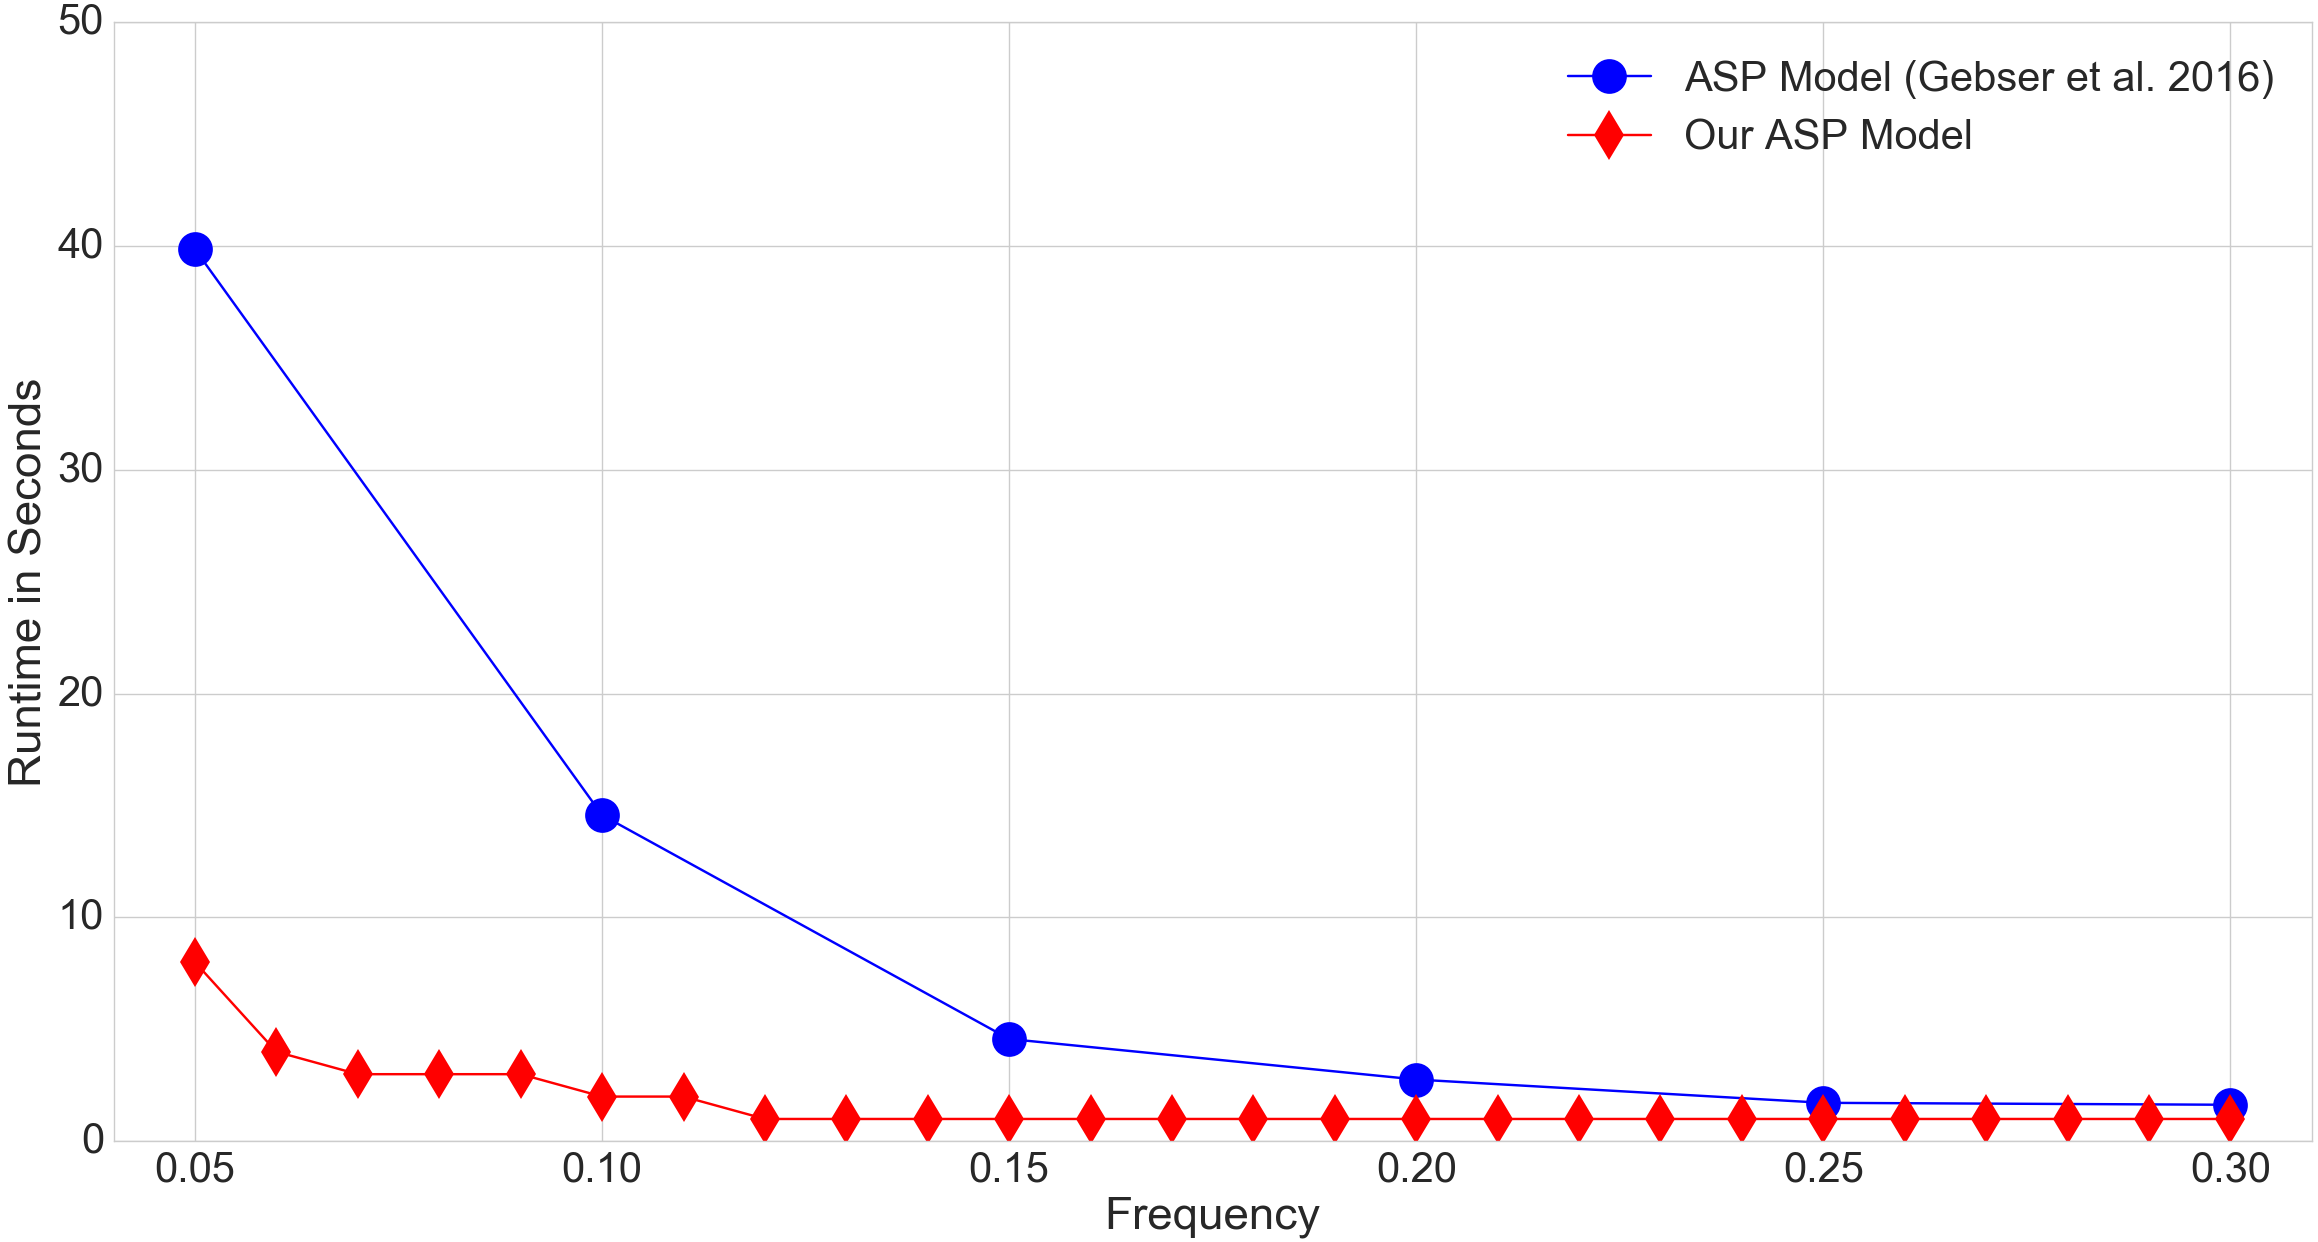
\includegraphics[width=\scalefigures\textwidth]{runtime_sequences_comparison.png}
   \caption{Comparing with ASP sequence model \parencite{DBLP:conf/ijcai/GebserGQ0S16} on the 200 generated sequences (closed)}
    \label{fig:sequence_comparison}
  \end{subfigure}
 \hfill
  \begin{subfigure}[t]{0.49\textwidth}
   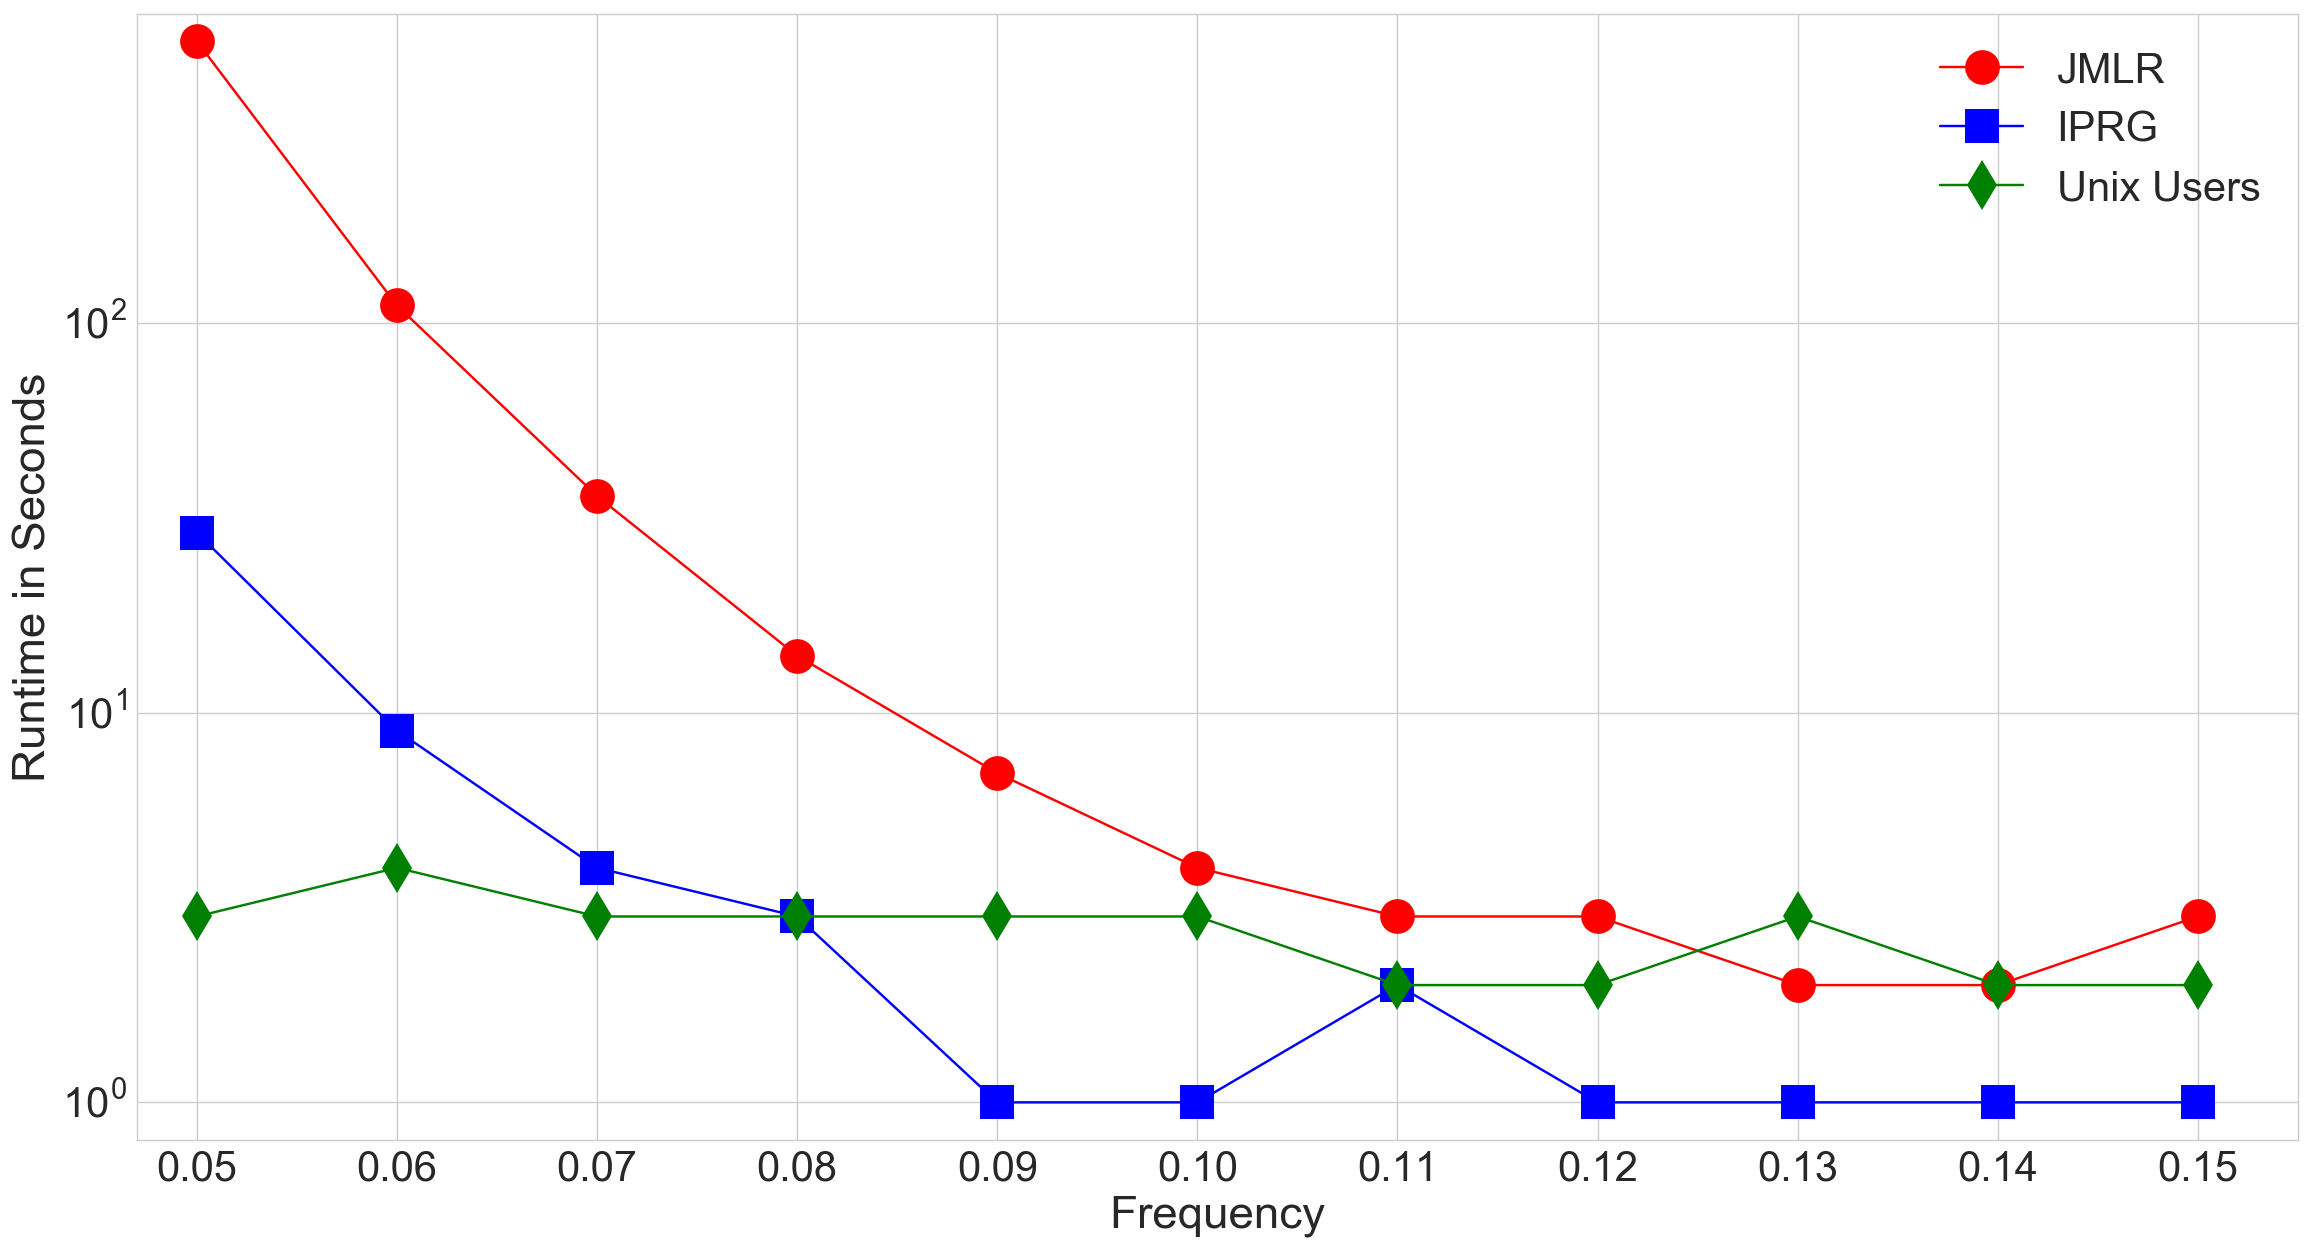
\includegraphics[width=\scalefigures\textwidth]{maximal.png}
   \caption{Maximal sequence patterns} %: JMLR, Unix Users and iPRG}
    \label{fig:maximal}
  \end{subfigure}
 \hfill
  \begin{subfigure}[t]{0.49\textwidth}
   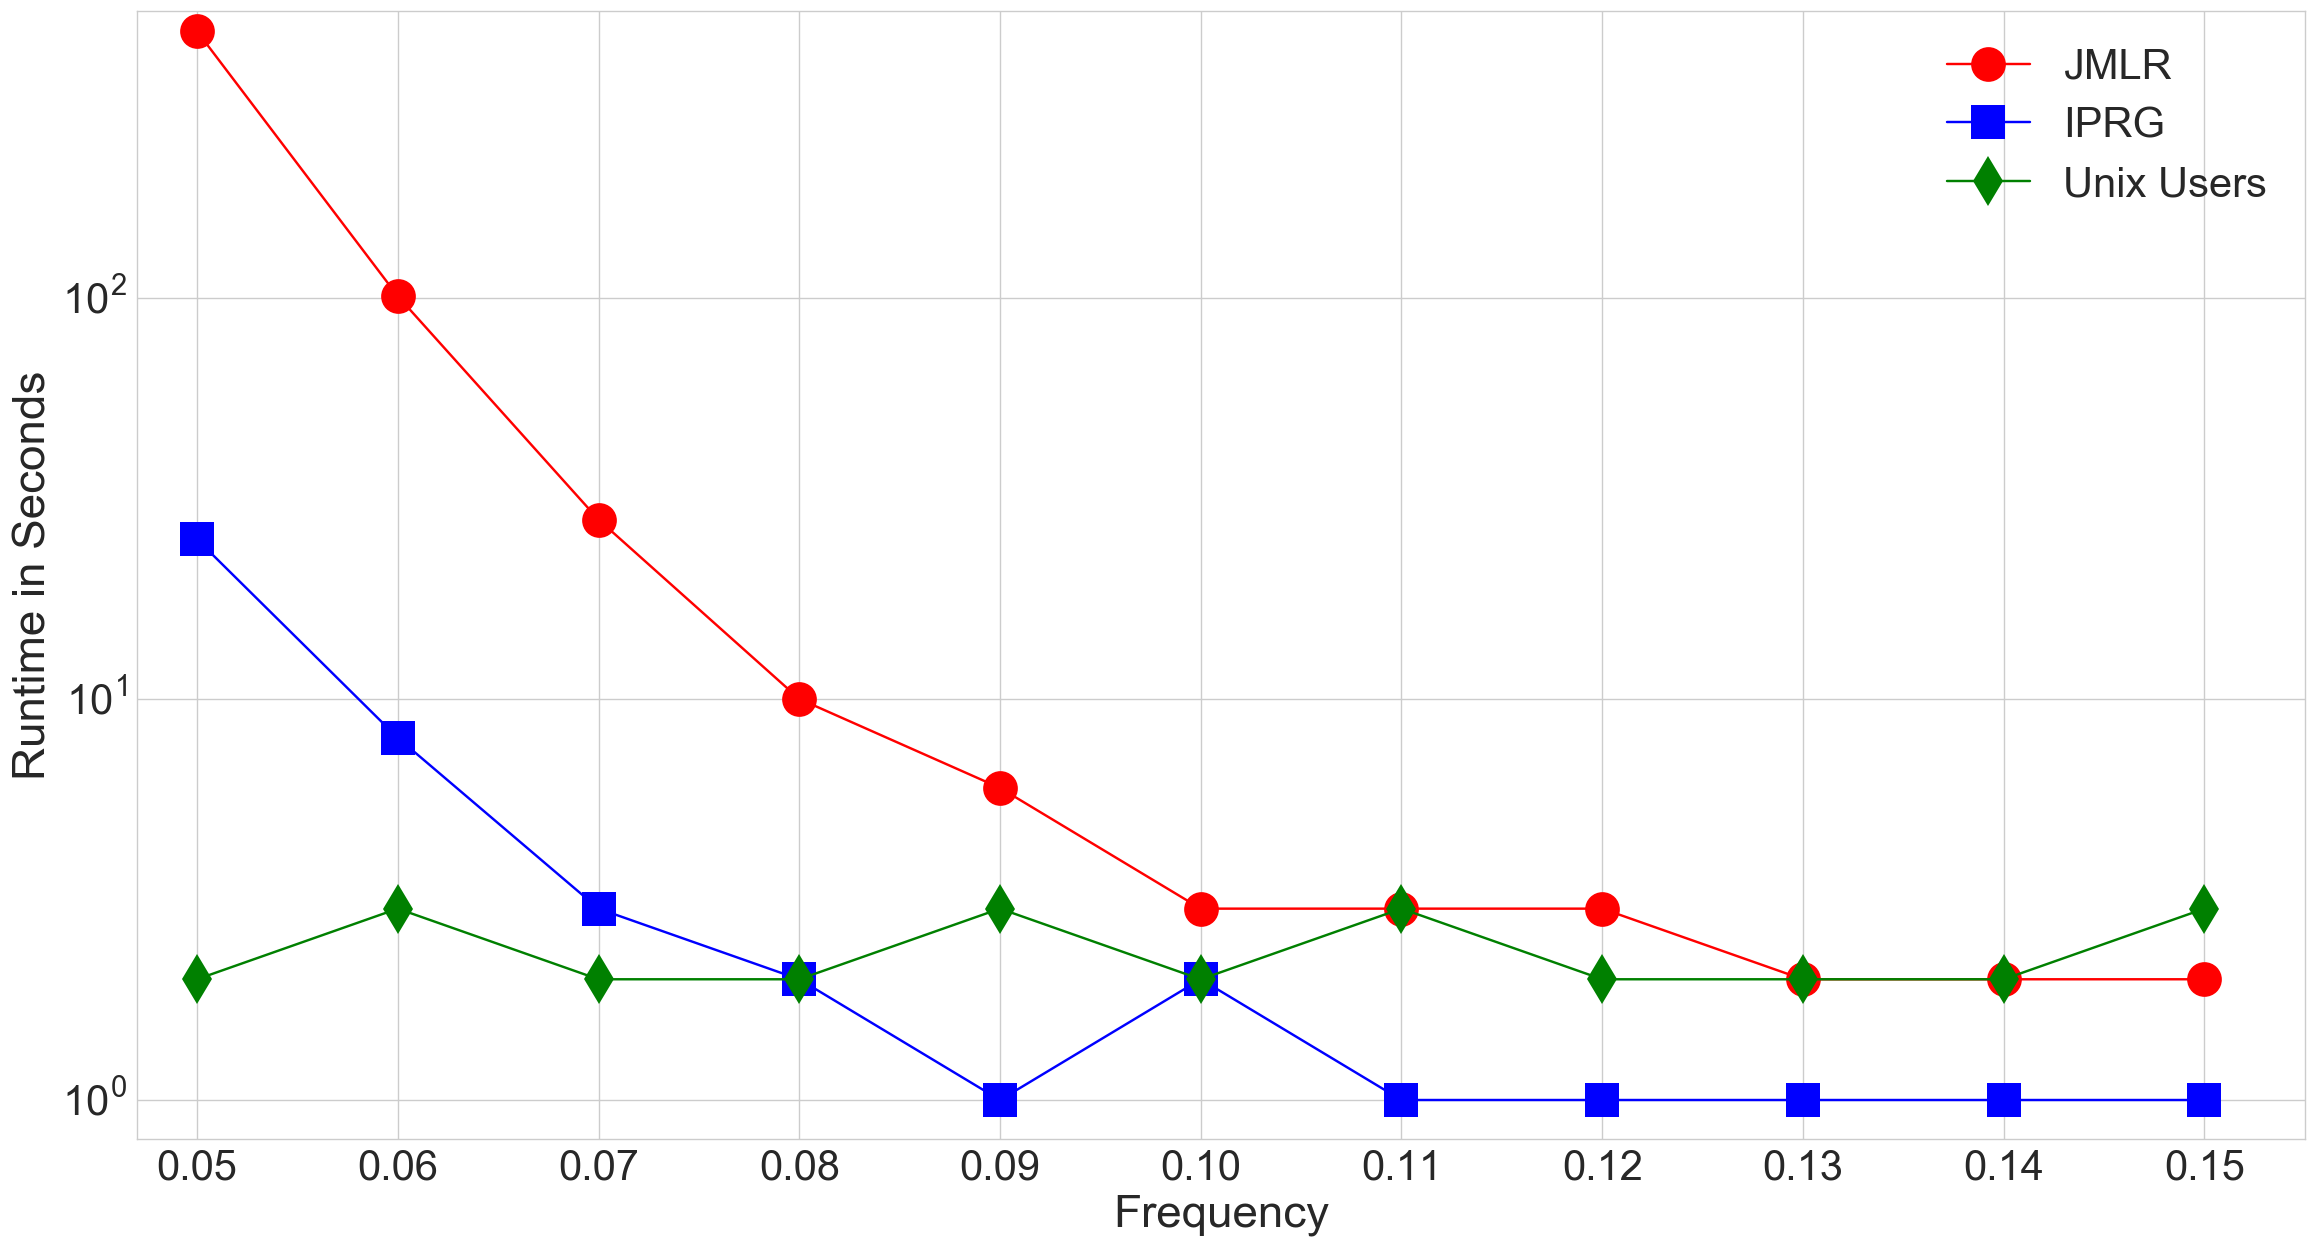
\includegraphics[width=\scalefigures\textwidth]{closed.png}
   \caption{Closed sequence patterns} %: JMLR, Unix Users and iPRG}
    \label{fig:closed}
  \end{subfigure}
\hfill
  \begin{subfigure}[t]{0.49\textwidth}
   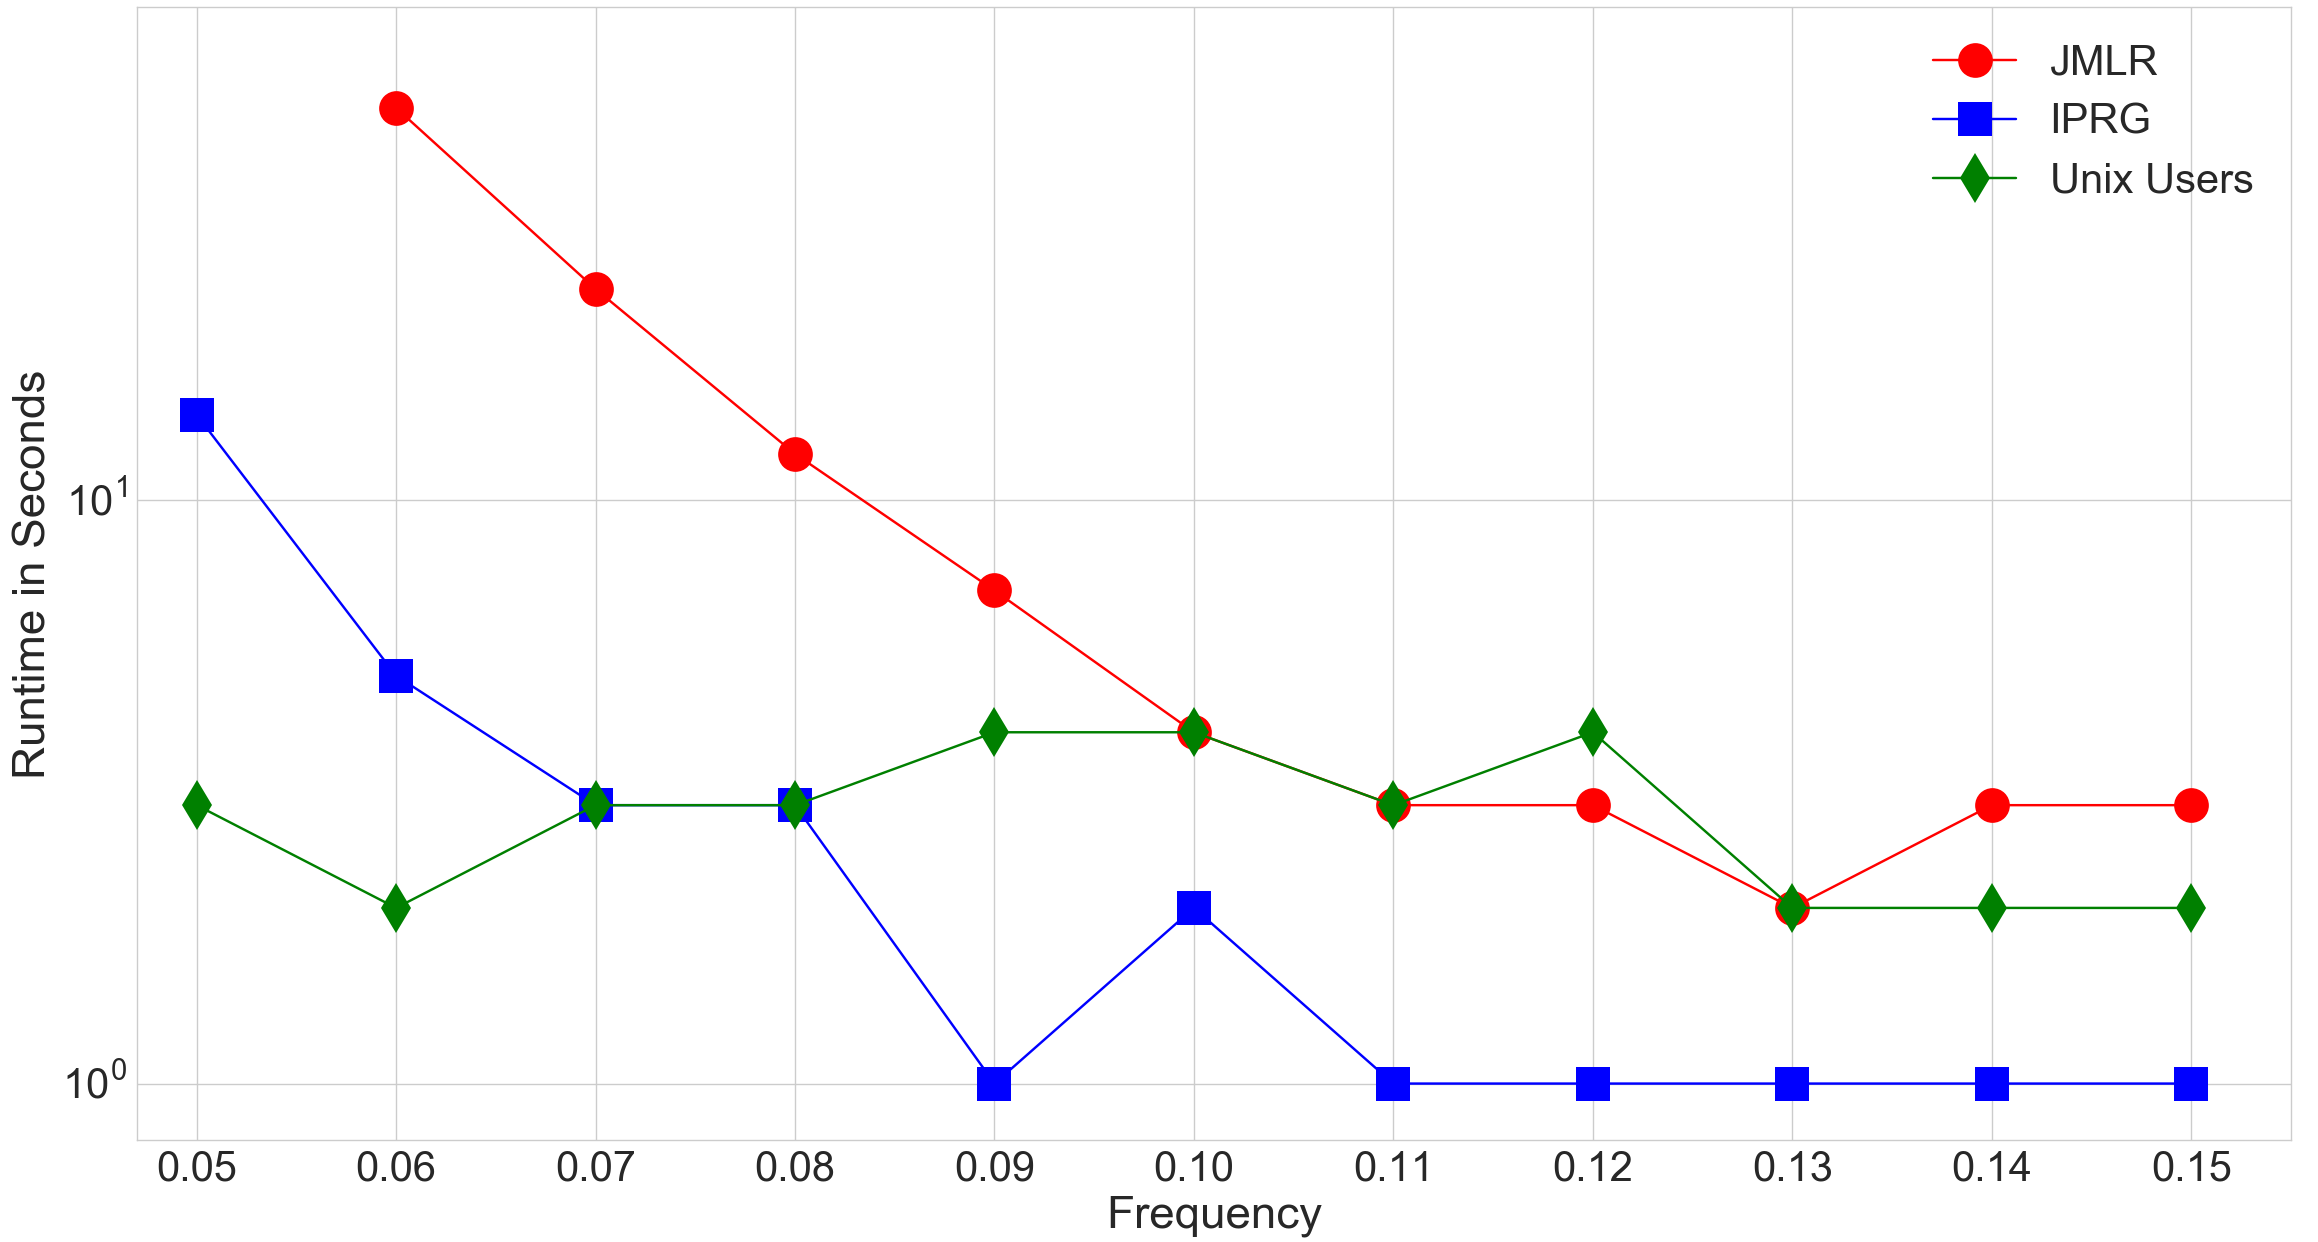
\includegraphics[width=\scalefigures\textwidth]{skyline.png}
   \caption{Skyline sequence patterns} %: JMLR, Unix Users and iPRG}
    \label{fig:skyline}
  \end{subfigure}
  \caption{Investigating \qone: comparison with pure ASP model (\ref{fig:sequence_comparison}) and maximal (\ref{fig:maximal}),  closed (\ref{fig:closed}), and skyline (\ref{fig:skyline}) sequence mining on  JMLR, Unix Users, and iPRG datasets.}
  \label{fig:qone}
\end{figure}

To investigate \qone, in Fig.~\ref{fig:sequence_comparison}, we compare the ASP model \parencite{DBLP:conf/ijcai/GebserGQ0S16} with our method on the default 200 sequence sample, generated by the tool\footnote{\url{https://sites.google.com/site/aspseqmining}} from \parencite{DBLP:conf/ijcai/GebserGQ0S16}. We %have to 
performed the comparison on the synthetic data, as the sequence-mining model \parencite{DBLP:conf/ijcai/GebserGQ0S16} failed to compute condensed representations on any of the standard sequence datasets for any support threshold value within the timeout. One can observe that our method consistently outperforms the purely declarative approach \parencite{DBLP:conf/ijcai/GebserGQ0S16} and the advantage naturally becomes more apparent for smaller frequency threshold values. %since within the time-limit of an hour the sequence-mining ASP model could not compute condensed representation on the datasets for any threshold value.
 
In Figs.~\ref{fig:maximal},~\ref{fig:closed} and~\ref{fig:skyline} (the point $0.05$ for JMLR is a timeout), we present the runtimes of our method for \emph{maximal, closed} and \emph{skyline} sequential pattern mining settings on JMRL, Unix Users and iPRG datasets. In contrast to \parencite{DBLP:conf/ijcai/GebserGQ0S16}, our method managed to produce results on all of these datasets for reasonable threshold values within a couple of minutes.
%(the runtime on Unix Users shows slight fluctuations within a couple of seconds). %\sergey{it is just runtime is low on that dataset, so 2 second fluctuations occur}). 
% The runtime of our method on datasets JMLR, Unix Users and iPRG %can be found 
% for \emph{closed}, \emph{maximal} and \emph{skyline} sequences are presented in Figure~\ref{fig:closed}, %\textit{maximal} in 
%  Figure~\ref{fig:maximal} and %\textit{skyline} in 
% Figure~\ref{fig:skyline} resp. Overall, we observe in Figure \ref{fig:qone} that our method provides better scalability and can be run within reasonable time on the real datasets, while covering the most popular condensed representation types as the model based only on ASP.

\begin{figure}[tb]
  \centering
  \begin{subfigure}[t]{0.49\textwidth}
   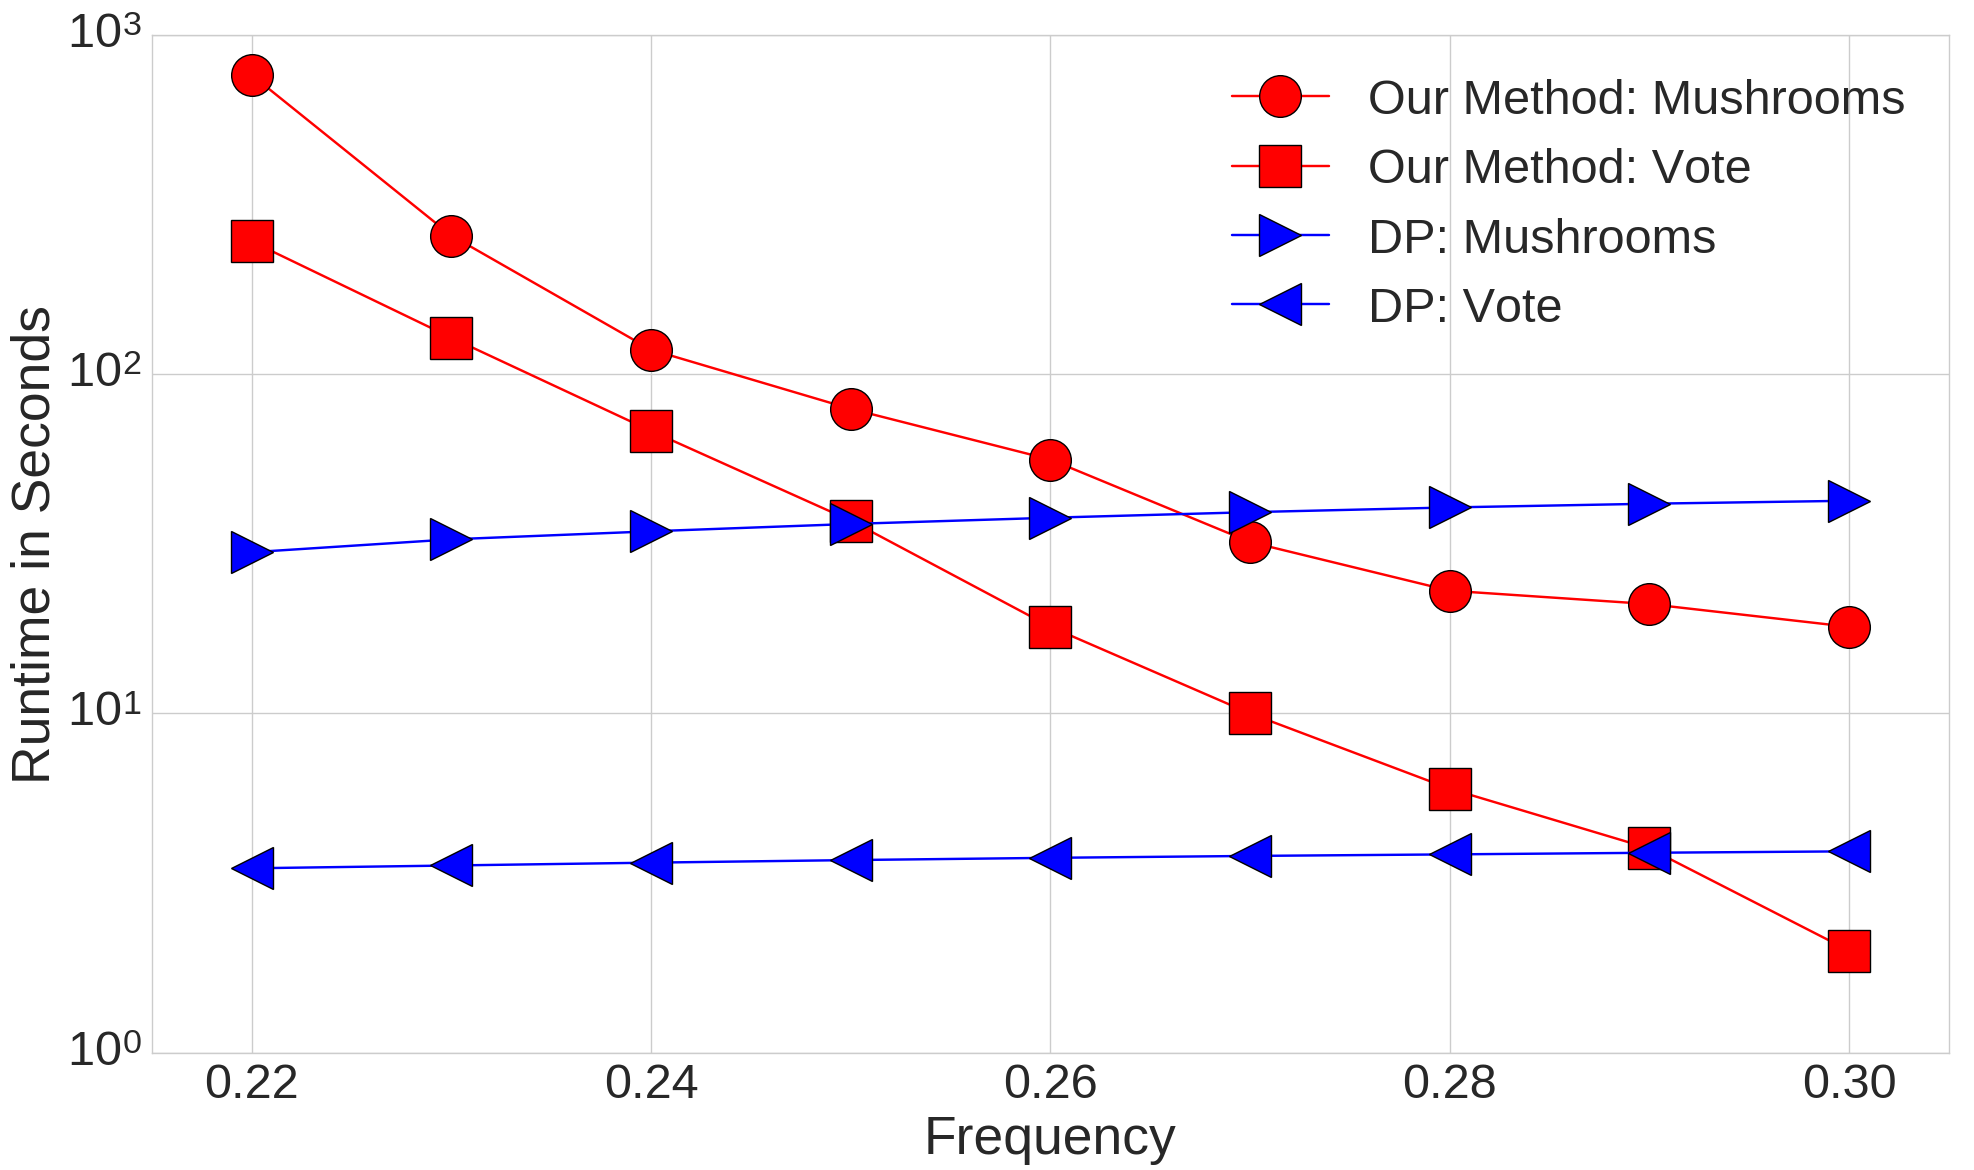
\includegraphics[width=\scalefigures\textwidth]{dp_maximal.png}
   \caption{Maximal itemset mining: comparing with DP on Vote and Mushrooms}
    \label{fig:dp_maximal}
  \end{subfigure}
 \hfill
  \begin{subfigure}[t]{0.49\textwidth}
   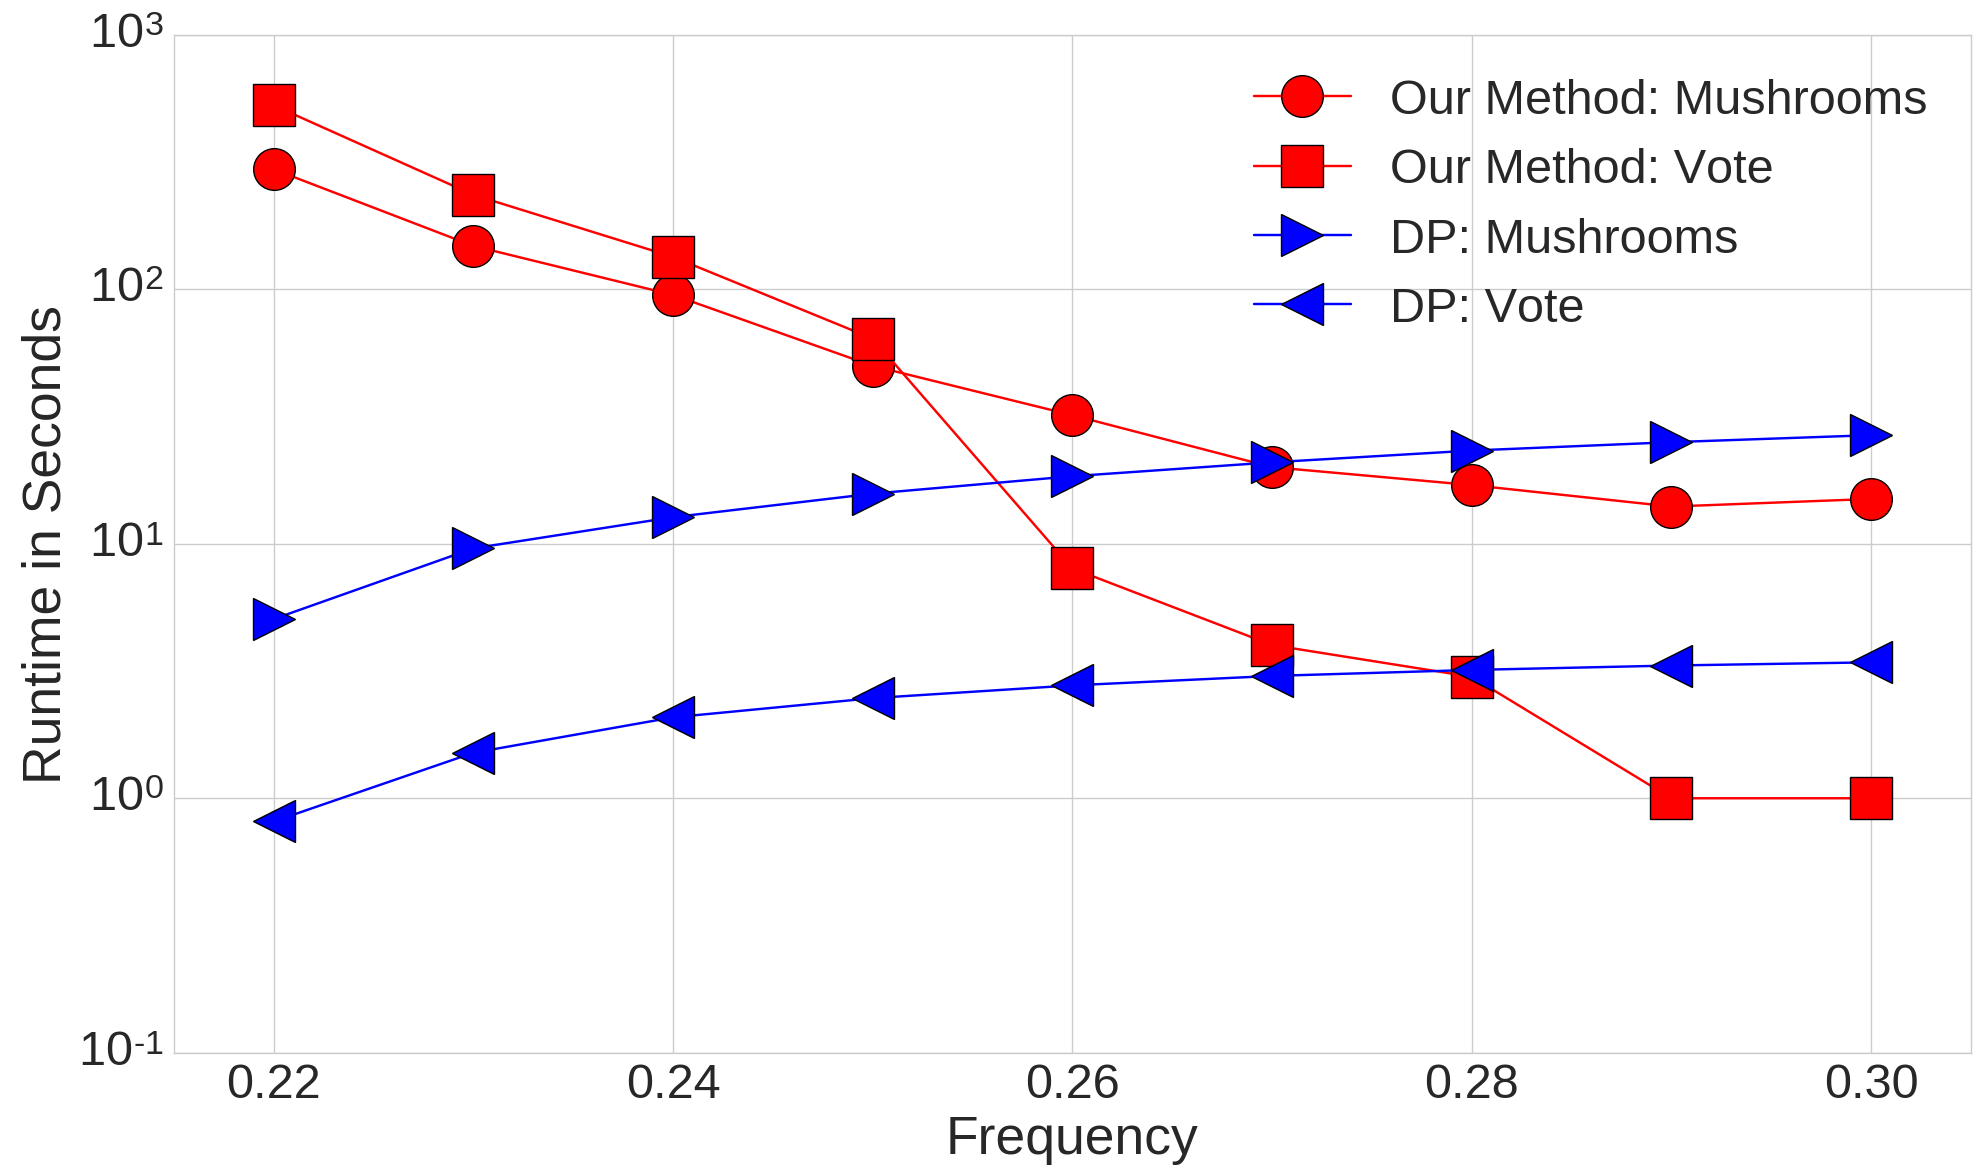
\includegraphics[width=\scalefigures\textwidth]{dp_closed}
   \caption{Closed itemset mining: comparing with DP on Vote and Mushrooms}
    \label{fig:dp_closed}
  \end{subfigure}
 \hfill
  \begin{subfigure}[t]{0.49\textwidth}
   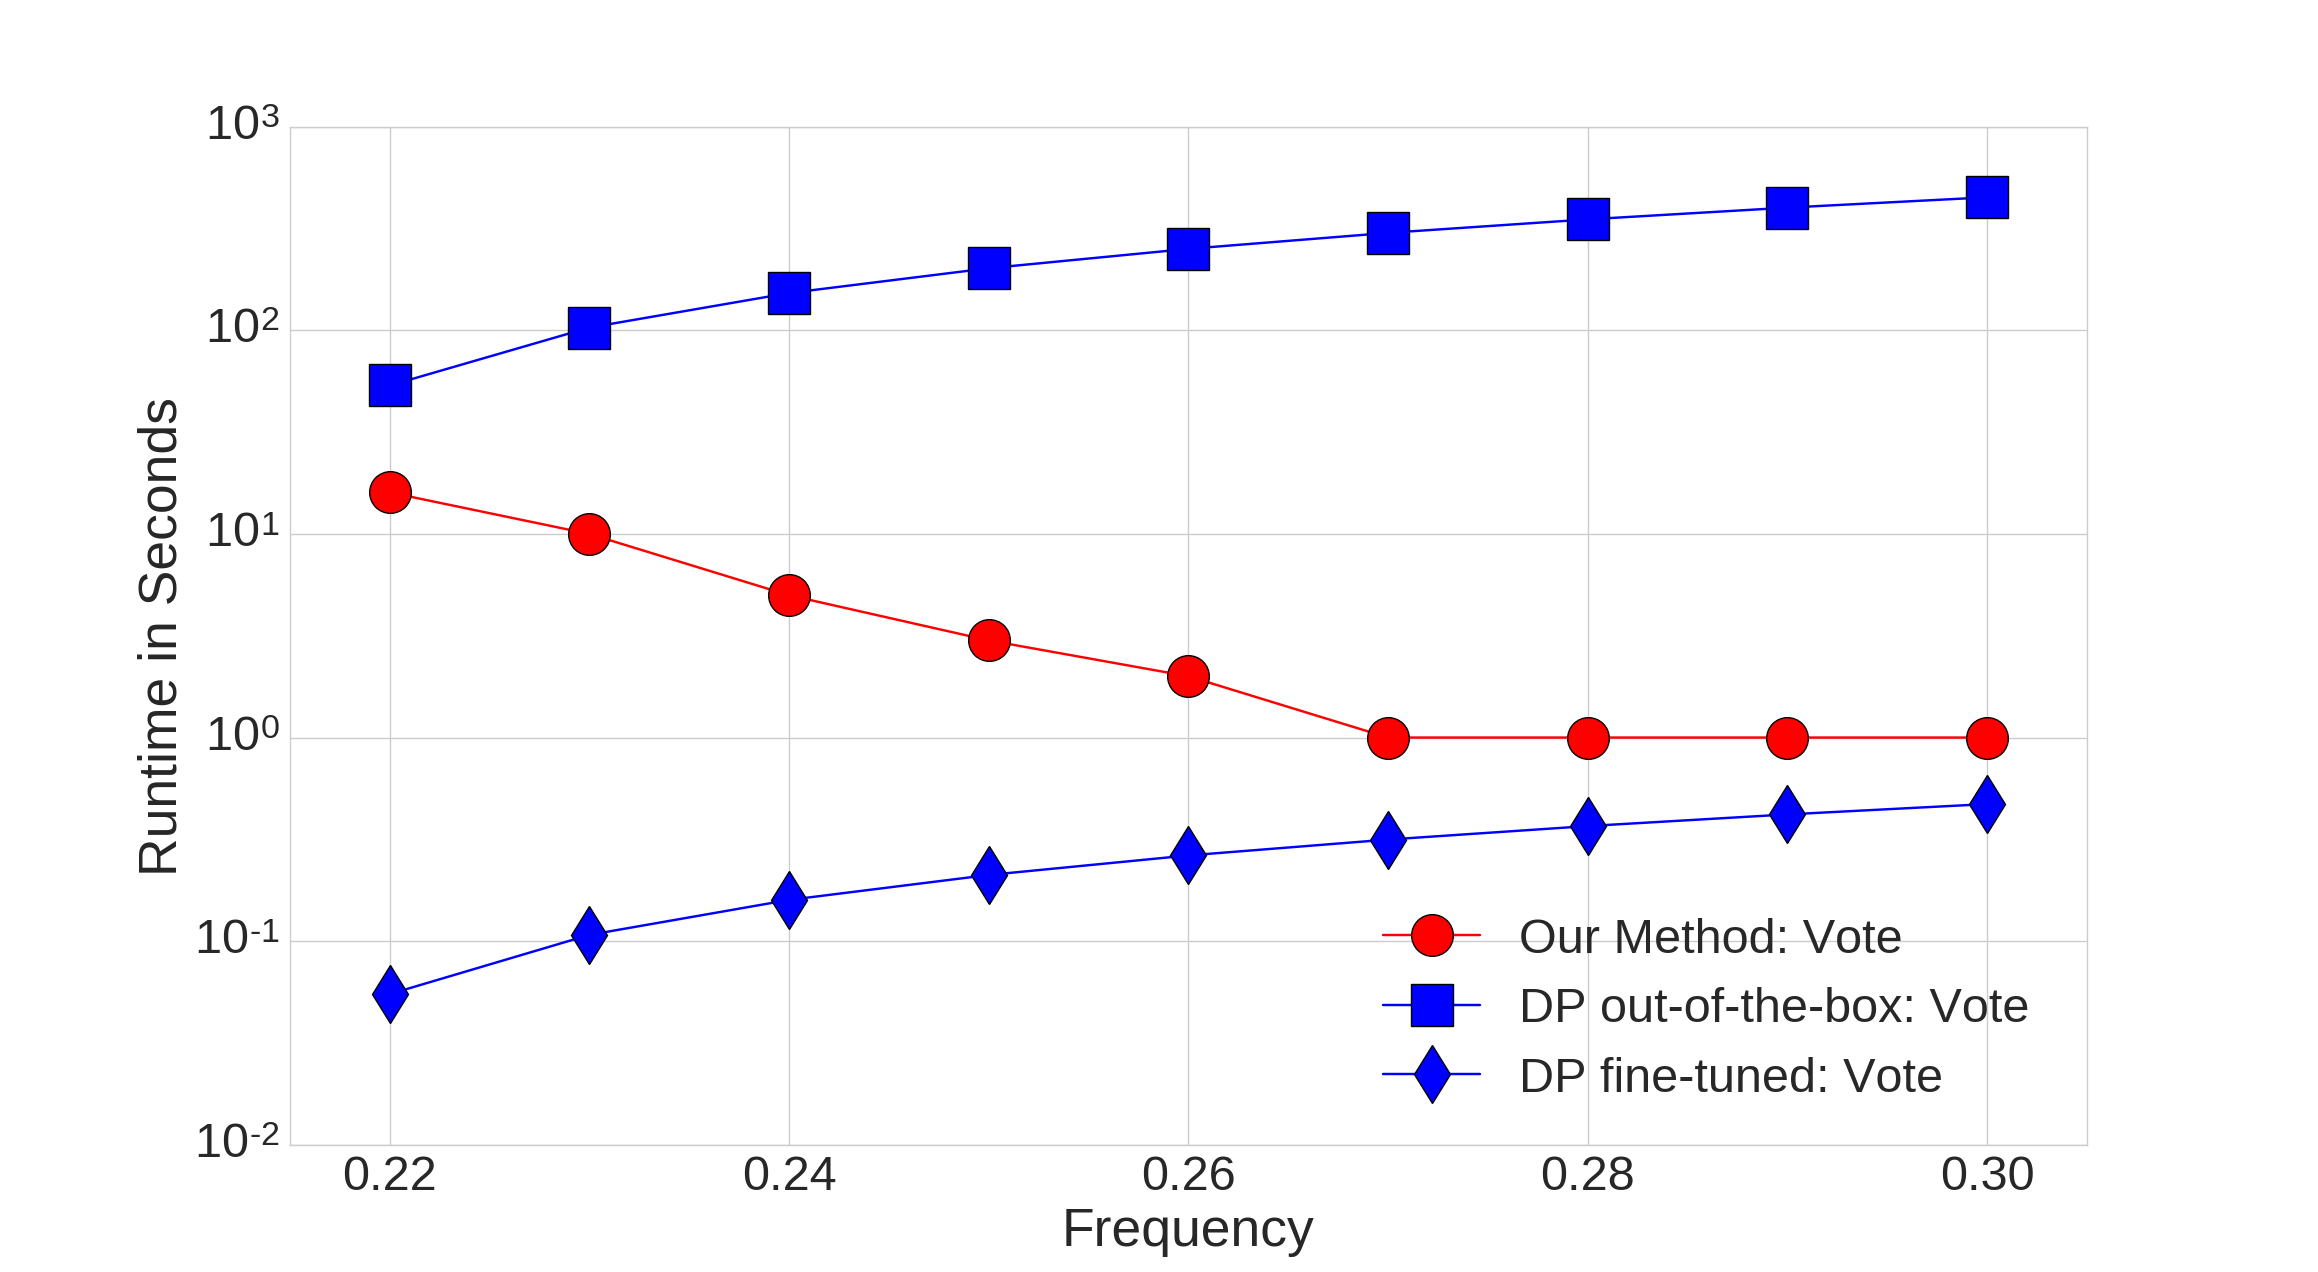
\includegraphics[width=\scalefigures\textwidth]{dp_skyline.png}
   \caption{Skyline itemset mining: comparing with out-of-the-box and fine-tuned DP on Vote}
    \label{fig:dp_skyline}
  \end{subfigure}
\hfill
  \begin{subfigure}[t]{0.49\textwidth}
   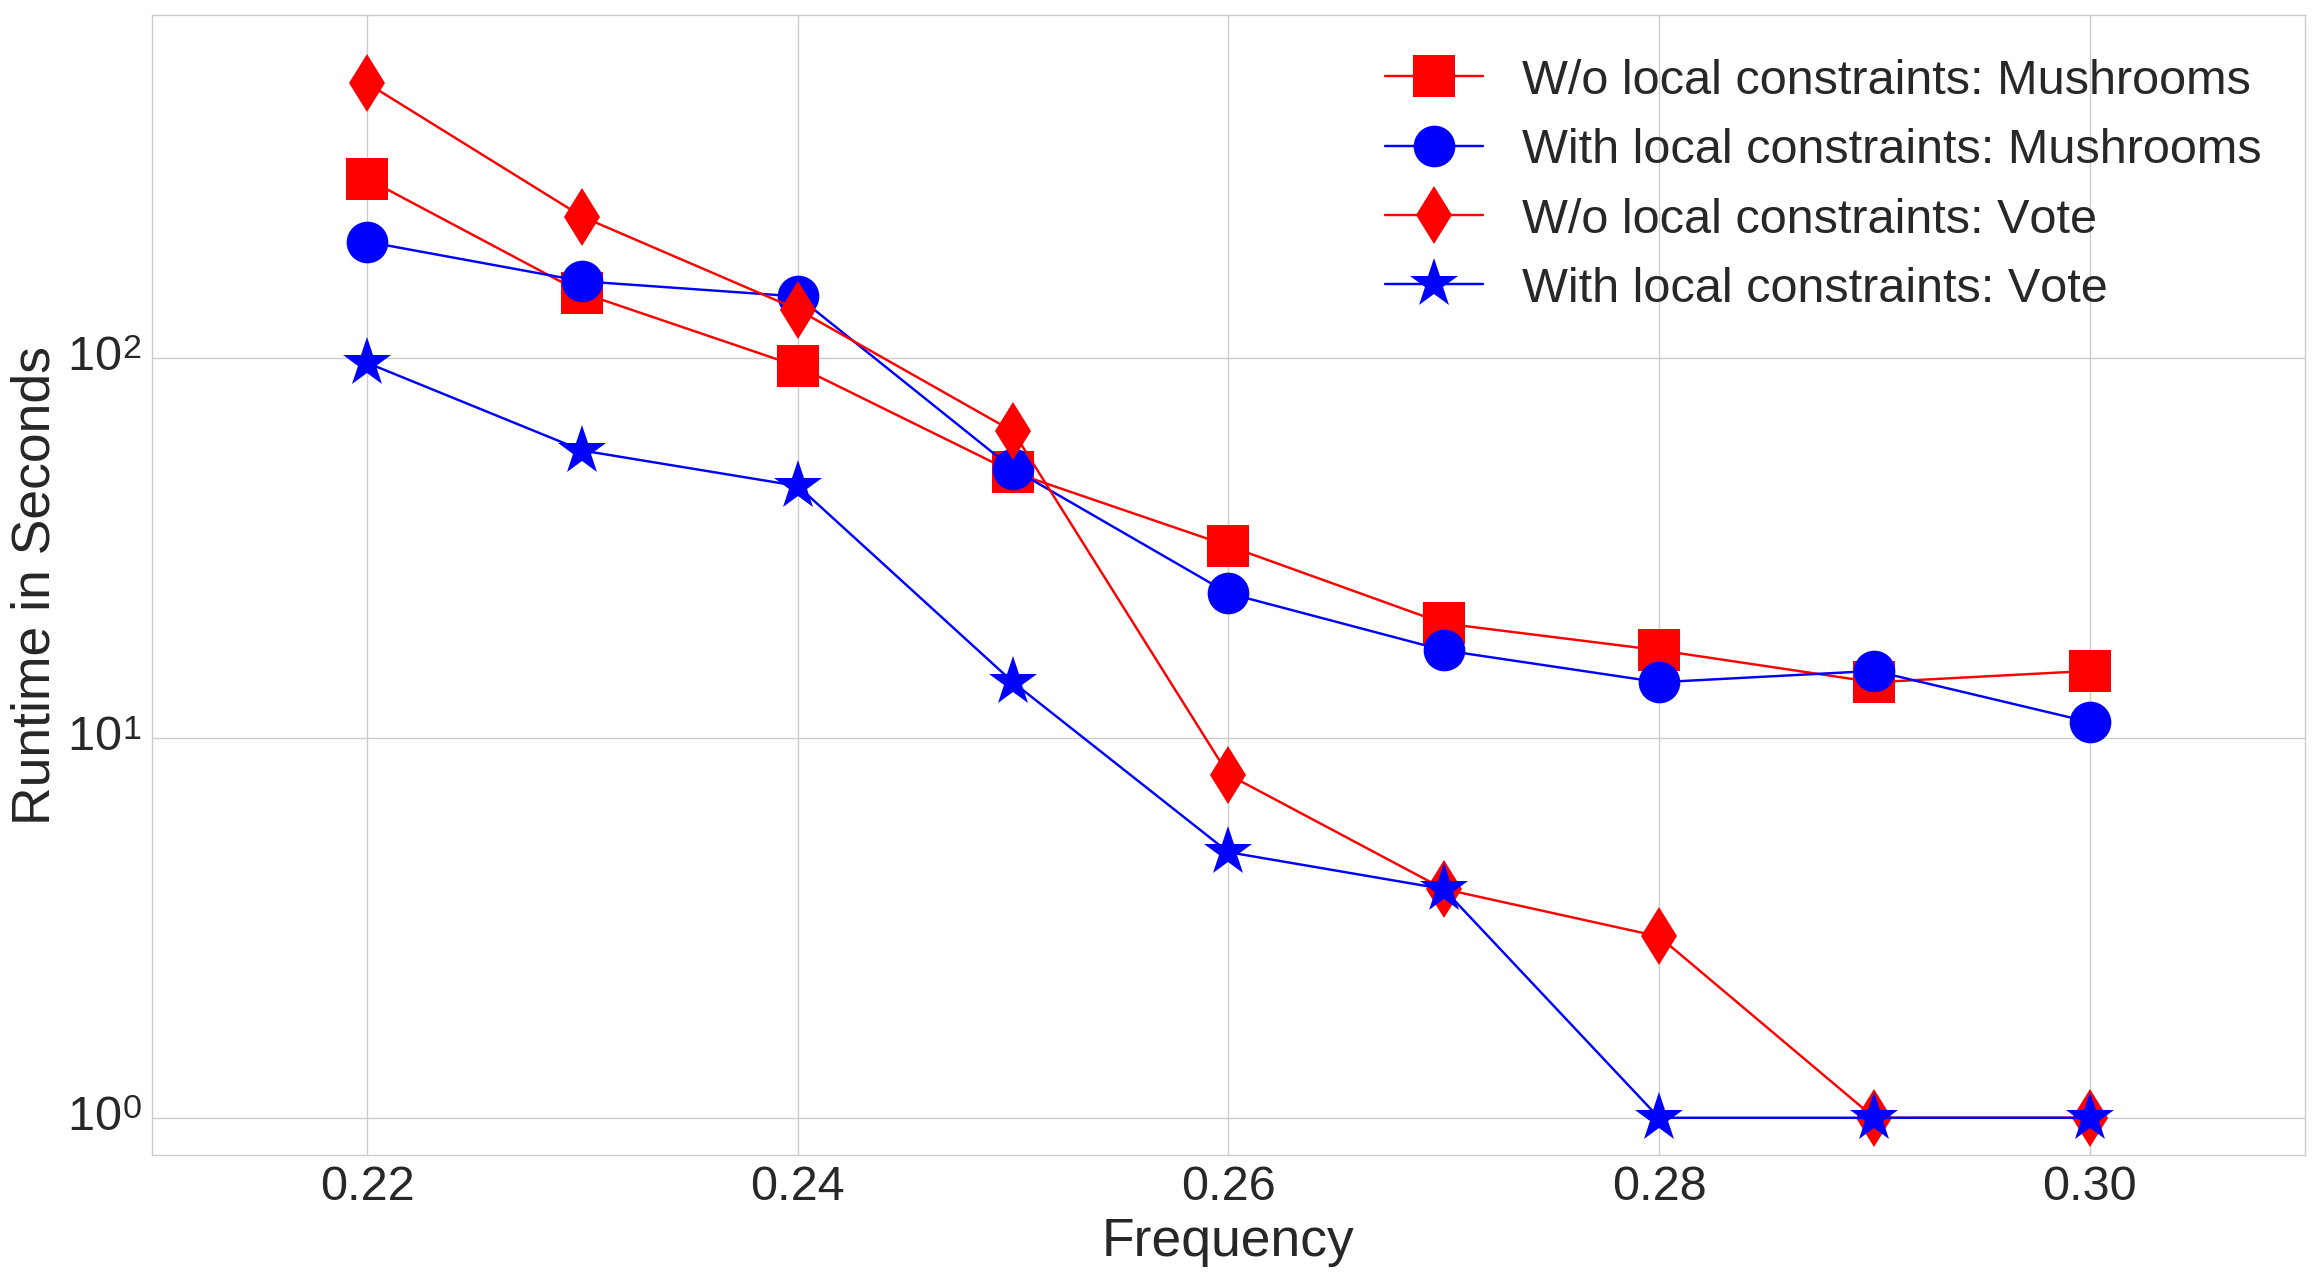
\includegraphics[width=\scalefigures\textwidth]{itemset_under_constraints.png}
   \caption{Closed itemset mining: our method with (w/o) local constraints on Vote and Mushrooms}%: local constraint enable faster propagation and speedup the search}
    \label{fig:local_constraints}
  \end{subfigure}
  \caption{Investigating \qtwo: comparison with DP \parencite{dp2013} (\ref{fig:dp_closed}, \ref{fig:dp_maximal}, \ref{fig:dp_skyline}); and \qthree: the effect of local constraints on runtime (\ref{fig:local_constraints})}
  \label{fig:qtwo_three}
\end{figure}


To investigate \qtwo, we compare out-of-the-box performance of DP \parencite{dp2013} with our approach on maximal, closed and skyline itemset mining problems using standard datasets Vote and Mushrooms. As we see in Figs.~\ref{fig:dp_maximal} and \ref{fig:dp_closed}, on average, DP is one-to-two orders of magnitude faster; this gap is, however, diminishing as the minimum frequency increases. %as the frequency grows. 
%What is more surprising, 
Surprisingly, our approach is significantly faster than DP out-of-the-box for skyline patterns (Fig.~\ref{fig:dp_skyline}); this holds also for the Mushrooms dataset, not presented here. 

Fine-tuning parameters of DP by changing the order in which operators are applied within the system (skyline+ option) allowed to close this gap. With this adaptation DP demonstrates one-to-two orders of magnitude better performance, as can be seen in Fig.~\ref{fig:dp_skyline}. However, fine-tuning such a system requires the understanding of its inner mechanisms or exhaustive application of all available options. 
% It is possible to fine-tune DP to change its behavior to close this gap. More specifically, we analyzed all options of DP and found that besides the default flag \textit{skyline} for skyline patterns, the option \textit{skyline+} is also available, which computes the same patterns but applies operators in a different order. Then DP 

To %investigate 
address \qthree we introduced three simple local constraints %into 
for the itemset mining setting from \qtwo: %. Namely, we used 
two size constraints $\textit{size(I)} > 2$ and $\textit{size(I)} < 7$ and a cost constraint: each item gets weight equal to its value with the maximal budget of $n$, which is set to $20$ in the experiments. % (Vote has 435 transactions and 48 binary items and Mushrooms has 8124 and 119 resp.). 

In Fig.~\ref{fig:local_constraints}, we present the results for closed itemset mining with and without local constraints (%other 
experiments with other global constraints demonstrate a similar runtime pattern and are not depicted here for space reasons). %One can see that 
Local constraints ensure %allow for 
better propagation and speed up the search. One of the key design features of our encoding is the filtering technique used to select candidate patterns among only valid patterns. Its effect can be clearly seen, e.g., for the Vote dataset in Fig.~\ref{fig:local_constraints}, where for certain frequencies the runtime gap is close to an order of magnitude.

In all experiments, Step 1 of our method contributes to less than 5\% of runtime. Overall, our approach can handle real world datasets for sequential pattern mining as demonstrated in \qone. In many cases %it 
its performance is %demonstrates performance 
close to the specialized mining languages, as % discussed 
shown in \qtwo. Finally, as demonstrated in \qthree various local constraints can be effectively incorporated into our encoding
%can 
bringing additional performance benefits. %from the local constraints 

\section{ASP-based Hybrid Mining Related Work}\label{sec:hybrid_relwork}

The problem of enhancing pattern mining by injecting various user-specified constraints has recently gained increasing attention. On the one hand, optimized dedicated approaches exist, in which some of the constraints are deeply integrated into the mining algorithm, e.g., \parencite{DBLP:conf/kdd/PeiH00}.  On the other hand, %purely 
declarative methods based on Constraint Programming \parencite{sky2014,DBLP:conf/cpaior/NegrevergneG15,DBLP:journals/corr/MetivierLC13}, SAT solving \parencite{DBLP:conf/pakdd/JabbourSS15,DBLP:conf/cikm/JabbourSS13} and ASP \parencite{DBLP:conf/lpnmr/Jarvisalo11,DBLP:conf/ijcai/GebserGQ0S16,DBLP:journals/corr/GuyetMQ14} have been proposed. 

Techniques from the last group are the closest to our work. However, in contrast to our method, they typically focus only on one particular pattern type and consider local constraints and condensed representations in isolation \parencite{DBLP:conf/dmkd/PeiHM00,clospan}. %(with exceptions 
The works \parencite{dp2013,DBLP:journals/ai/GunsDNTR17} focused on CP-based rather than ASP-based itemset mining and did not take into account sequences unlike we do. The authors of \parencite{DBLP:conf/ijcai/GebserGQ0S16} studied declarative sequence mining with ASP, but in contrast to our approach, optimized algorithms for frequent pattern discovery are not exploited in their method.
A theoretical framework for structured pattern mining was proposed in \parencite{DBLP:conf/aaai/GunsPN16}, whose main goal was to formally define the core components of the main mining tasks and compare dedicated mining algorithms to their declarative versions. While generic, this work did not take into account local and global constraints and neither has it been implemented.

In \parencite{DBLP:conf/lpnmr/Jarvisalo11,DBLP:conf/ijcai/GebserGQ0S16}, purely declarative ASP methods have been considered; unlike our approach, they do not admit integration of optimized mining algorithms and thus %which 
lack 
practicality. In fact, the need for such an integration in the context of complex structured mining was even explicitly stated
in \parencite{query_mining_ilp} and in \parencite{KR_Graphs}, which study formalizations of graph mining problems using logical means. 

% Paramonov et al. presents an initial formalization of graph mining using logic programming in \parencite{query_mining_ilp} and Van der Hallen et al. \parencite{KR_Graphs} cover theoretical and practical problems of modeling graph mining using pure logical models indicating that higher order reasoning or a hybrid approach is needed to model complex structured mining problems in general case.
\section{Hybrid Approach Conclusion}

We have presented a hybrid approach for condensed itemset and sequence mining, which uses the optimized dedicated algorithms to determine the frequent patterns and post-filters them using a declarative ASP program. The idea of exploiting ASP for pattern mining is not new; it was studied for both itemsets and sequences. However, unlike previous methods we made steps towards optimizing the declarative techniques by making use of the existing specialized methods and also integrated the dominance programming machinery in our implementation to allow for combining local and global constraints on a generic level.


%\section{Future Work}\label{sec:futwork}
One of the possible future directions is to generalize the proposed approach into an iterative technique, where dedicated data mining and declarative methods are interlinked and applied in an iterative fashion. More specifically, all constraints can be split into two parts: those that can be effectively handled using declarative means and those for which specialized algorithms are much more scalable. Answer set programs with external computations \parencite{hp} possibly could be exploited in this mining context. % Then the pattern selection can be done iteratively. For example, let the constraints be given as (1) frequency (2) closed (3) length (4) gap size. We can first apply dedicated algorithms to get patterns that satisfy the frequency constraint. Then select only closed patterns among them using declarative means. After that the original transaction database can be filtered by removing transactions, in which none of the computed closed patterns appears. Then the final check can be applied to test the gap constraint. In other words our hybrid approach can be generalized resulting in the iterative application of the dedicated algorithms and declarative pruning methods.


Another promising but challenging research stream concerns the integration of data \emph{decomposition} techniques into our approach. Here, one can divide a given dataset into several parts, such that the frequent patterns are identified in these parts separately, and then the results are combined.  % In fact decomposition can be performed at different levels. First possibility is to split the original dataset into components and then apply our hybrid approach on each component separately. Second option would be perform data splitting on the pattern level, i.e., once the frequent patterns are computed, we could come up with their splitting and then perform post-processing on every pattern group considered individually. Yet combinations of the two strategies are possible.

%Other ideas: exploit modular ASP, maybe 
Orthogonal to this, materialization of the presented ideas on other pattern types including graphs and sequences of itemsets instead of sequences of individual symbols is an interesting future direction. 


%%%%%%%%%%%%%%%%%%%%%%%%%%%%%%%%%%%%%%%%%%%%%%%%%%
% Keep the following \cleardoublepage at the end of this file, 
% otherwise \includeonly includes empty pages.
\cleardoublepage


